\documentclass[reprint,aps,pre,amsmath,amssymb,superscriptaddress,showpacs]{revtex4-1}
\usepackage{graphicx}
\usepackage{hyperref}
\usepackage{color}

\newtheorem{definition}{Definition}

\begin{document}

\title{Local network evolution rules drive shortest path multiplicity}

\author{Alexei Vazquez}
\email{alexei@nodeslinks.com}
\affiliation{Nodes \& Links Ltd, Salisbury House, Station Road, Cambridge, CB1 2LA, UK}

\begin{abstract}
The shortest path multiplicity is an important metric of complex networks. The shortest path multiplicity of real networks is high and it correlates with their community structure. Since local network evolution induces network communities, it is possible that a high shortest path multiplicity is the natural expectation of local evolution rules. Here I demonstrate, by means of numerical simulations, that this is indeed the case.
\end{abstract}

\maketitle

\section{Introduction}

The fundamental question of network science is to determine the minimum set of properties and models to explain what we observe in real networks. New discoveries should be subject to the scrutiny of existing concepts. That is the case of the  recent observation by Deng {\em et al} \cite{deng2026multipath}, a correlation between the number of communities and the density of multiple shortest paths in real networks. This correlation could be the consequence of an upstream factor that causes both features. And it turns out that there is an obvious candidate: local evolution rules.

Local network evolution rules are node/link addition mechanisms of network growth \cite{vazquez03local}. Local rules are inspired by the natural evolution of real networks. Web pages are created by copying other pages \cite{kleinberg99}. We cite references that we found reading another publication \cite{vazquez01rs}. Friends of friends become friends \cite{growing_social_networks_jin01}.  Proteins increase their connectivity when their interacting partners are duplicated \cite{vazquez03dup, pastor-satorras03}. Local evolution rules lead to the emergence of network communities: beyond a certain network size we can warrant that the network will exhibit communities \cite{vazquez2025local}. These communities are not written in the network evolution rules. Yet they are imputed by the state of the art methods to detect network communities.

Local evolution rules induce the formation of short cycles and cycles tend to increase the shortest path multiplicity. Therefore, I raise the hypothesis that the high shortest path multiplicity of real networks is rooted on their local growth dynamics. Furthermore, since those local rules induce the formation of networks communities, that would explain the association between shortest path multiplicity and network communities as well.

In this work I investigate this hypothesis by means of numerical simulations. In the Sec. \ref{methods} I introduce different models of growing networks with local rules and the methods used to quantify their properties. In Sec. \ref{random} I characterize random networks without local structures to set the baseline expectation. In Sec. \ref{local} I characterize the networks generated by local rules. The concluding remarks are reported in Sec. \ref{conclusions}.

\section{Methods}
\label{methods}

The computer code related to these methods is available at \href{https://github.com/av2atgh/ramsey_netcom}{github.com/av2atgh/ramsey\_netcom}.

\subsection{Local models}

Local search $LS(n, d)$. {\em Initial condition}. The network is started with two connected nodes. Evolution rule: A new node is added and a $d$-step random walk is performed from a randomly selected node in the current network. The new node is connected to all
visited nodes. This model has preferential attachment because the probability that a node is visited, beyond the entry node, is proportional to the current nodes degrees. Consequently it generate networks with a power law degree distribution. The $LS(n, d)$ networks have a
high clustering coefficient. At least 1 triangle, between the entry point and next neighbor visited, is formed at every node addition. For $d=1$ this model is equivalent to the triadic closure model \cite{growing_social_networks_jin01, communities_bianconi_2014}.

Duplication split $DS(n, q)$. {\em Initial condition}: The network is started with two connected nodes. {\em Evolution rule}: A new node $i$ is added to the network and a node in the current network is selected at random, node $j$. With probability $q$, $i$ becomes a duplicate of $j$ with links from $i$ to all neighbors of $j$. Otherwise, a link between $j$ and a randomly selected neighbor of $j$, node $k$, is split. The edge $(j, k)$ is removed and new edges $(i, j)$ and $(i, k)$ are created. This model has preferential attachment because, for the duplication rule, the probability that a node neighbor is duplicated is proportional to the node degree. The duplication rule does not make triangles and the split rule breaks triangles if they would exist. The main motif of this model is the formation of squares (cycles of length 4) between any two neighbors of the reference node $j$ and its duplicate $i$.

Bubble model $BB(n, L)$. {\em Initial condition}: The network is started with two connected nodes. {\em Evolution rule}: A chain of $L$ new nodes is added to the network. The two nodes at the chain ends are attached to the ends of an existing link, creating a cycle of length $L+2$. $BB(n, 1)$ is equivalent to an earlier Dorogovtsev-Mendes model where new nodes are connected to both ends of a randomly chosen link by two undirected links \cite{dorogotsev2001link}. The model has preferential attachment because the probability that a node is at the end of the selected link is proportional to its degree. The main network motif are the cycles of length $L+2$ created by the evolution rule.

All these models have a finite Ramsey community number $r_\kappa$, the minimum graph size that guarantees the emergence of network communities with almost certainty \cite{vazquez2025local}.

\subsection{Network communities}

The network communities are inferred using the stochastic block model implemented in graph-tool (\verb|graph_tool.inference.minimize_blockmodel_dl|, with default parameters) \cite{peixoto_graph-tool_2014}. This stochastic block model finds the community structure with the minimum description length \cite{peixoto2024networkreconstructionminimumdescription}. In that sense, it gives as output the optimal number of communities $\kappa$ and the partition of the nodes into communities. The average of $\kappa$ is calculated from 100 realizations of network creation plus network community inference.

An important parameter is the correction for the network degree sequence, \verb| deg_corr: bool (optional, default: True)|. Some of the networks investigated have power law degree distributions, and therefore I use the degree-corrected version of the stochastic block model (default option). Similar results are obtained using the Infomap method implemented in the package with the same name \cite{mapequation2025software}, as previously shown \cite{vazquez2025local}.

\subsection{Network rewiring}

For network rewiring, I use the standard configuration model implemented with \verb|graph_tool.generation.random_rewire| with default parameters. The configuration algorithm rewires the network links preserving the degree distribution \cite{configuration_method_park_2004}.

\subsection{Shortest path multiplicity}

To determine the path multiplicity $\mu_{ij}(G)$ between a pair of nodes $(i, j)$ in graph $G$, I use the graph-tool method \verb|graph_tool.count_shortest_paths(G, i, j)| with default parameters.

Given a graph generator $f_G$, I calculate the average shortest path multiplicity $\langle \mu\rangle$ as the average over every pair of nodes and over 100 realizations of $G$.

\begin{figure}
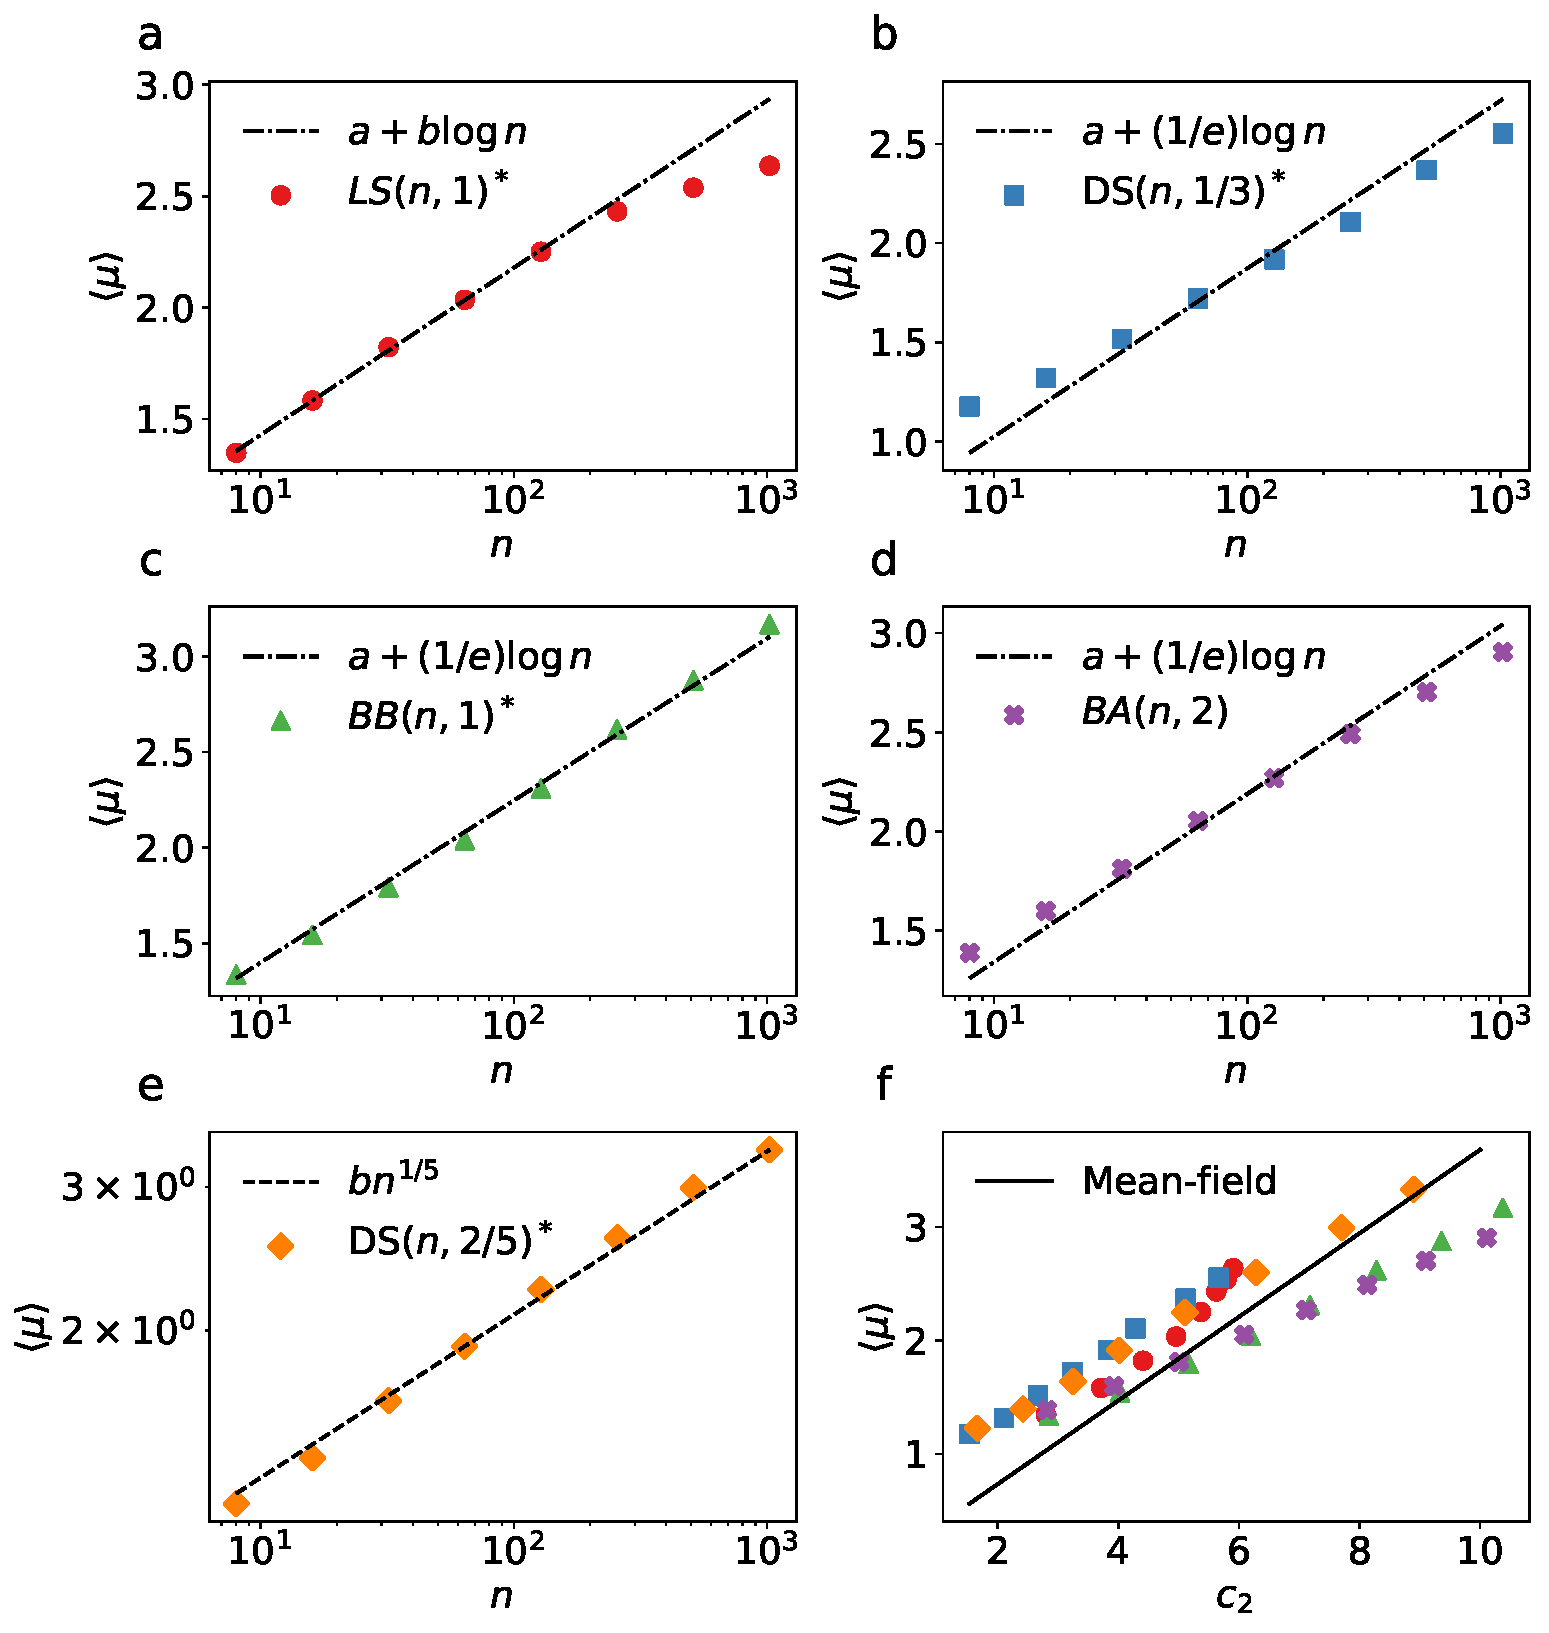
\includegraphics[width=3.4in]{fig1.pdf}
\caption{Scaling between the average shortest path multiplicity $\langle \mu\rangle$ and the network size $n$ for randomized networks. The networks were generated using the local rule indicated in the legend and then randomized by the degree preserving link rewiring. The lines highlight the logarithmic scaling.}
\label{fig_randomized}
\end{figure}

\section{Non-structured networks}
\label{random}

Dong {\em et al} \cite{dong2025multi} have estimated the network size scaling of the average shortest path multiplicity  for the Erd\"os-R\'enyi random graph model $ER(n, p)$, denoted by $\langle \mu\rangle_{ER}$. In the dense regime, $p$ near and above 0.1, $\langle \mu\rangle_{ER}$ scales linearly with $n$. However, real networks are sparse, corresponding to $p\sim1/n$.

To investigate sparse random networks, we can use as starting point the local rule models and then we apply the degree preserving link rewiring method. Figure \ref{fig_randomized} shows the average shortest path multiplicity $\langle \mu\rangle$ as a function of the network size $n$, the number of nodes. For all the sparse random networks tested there is a logarithmic growth
%
\begin{equation}
\langle \mu\rangle_{S,0} = a + b\log n,
\label{mu_rnd} 
\end{equation}
%
as it is emphasized by the fitted line in the semi-log plot. That is indeed slower than the linear dependency for the Erd\"os-R\'enyi graphs in the dense regime. The subscript {S0} stands for sparse network (S) and non-structured network (0). 

\begin{figure}
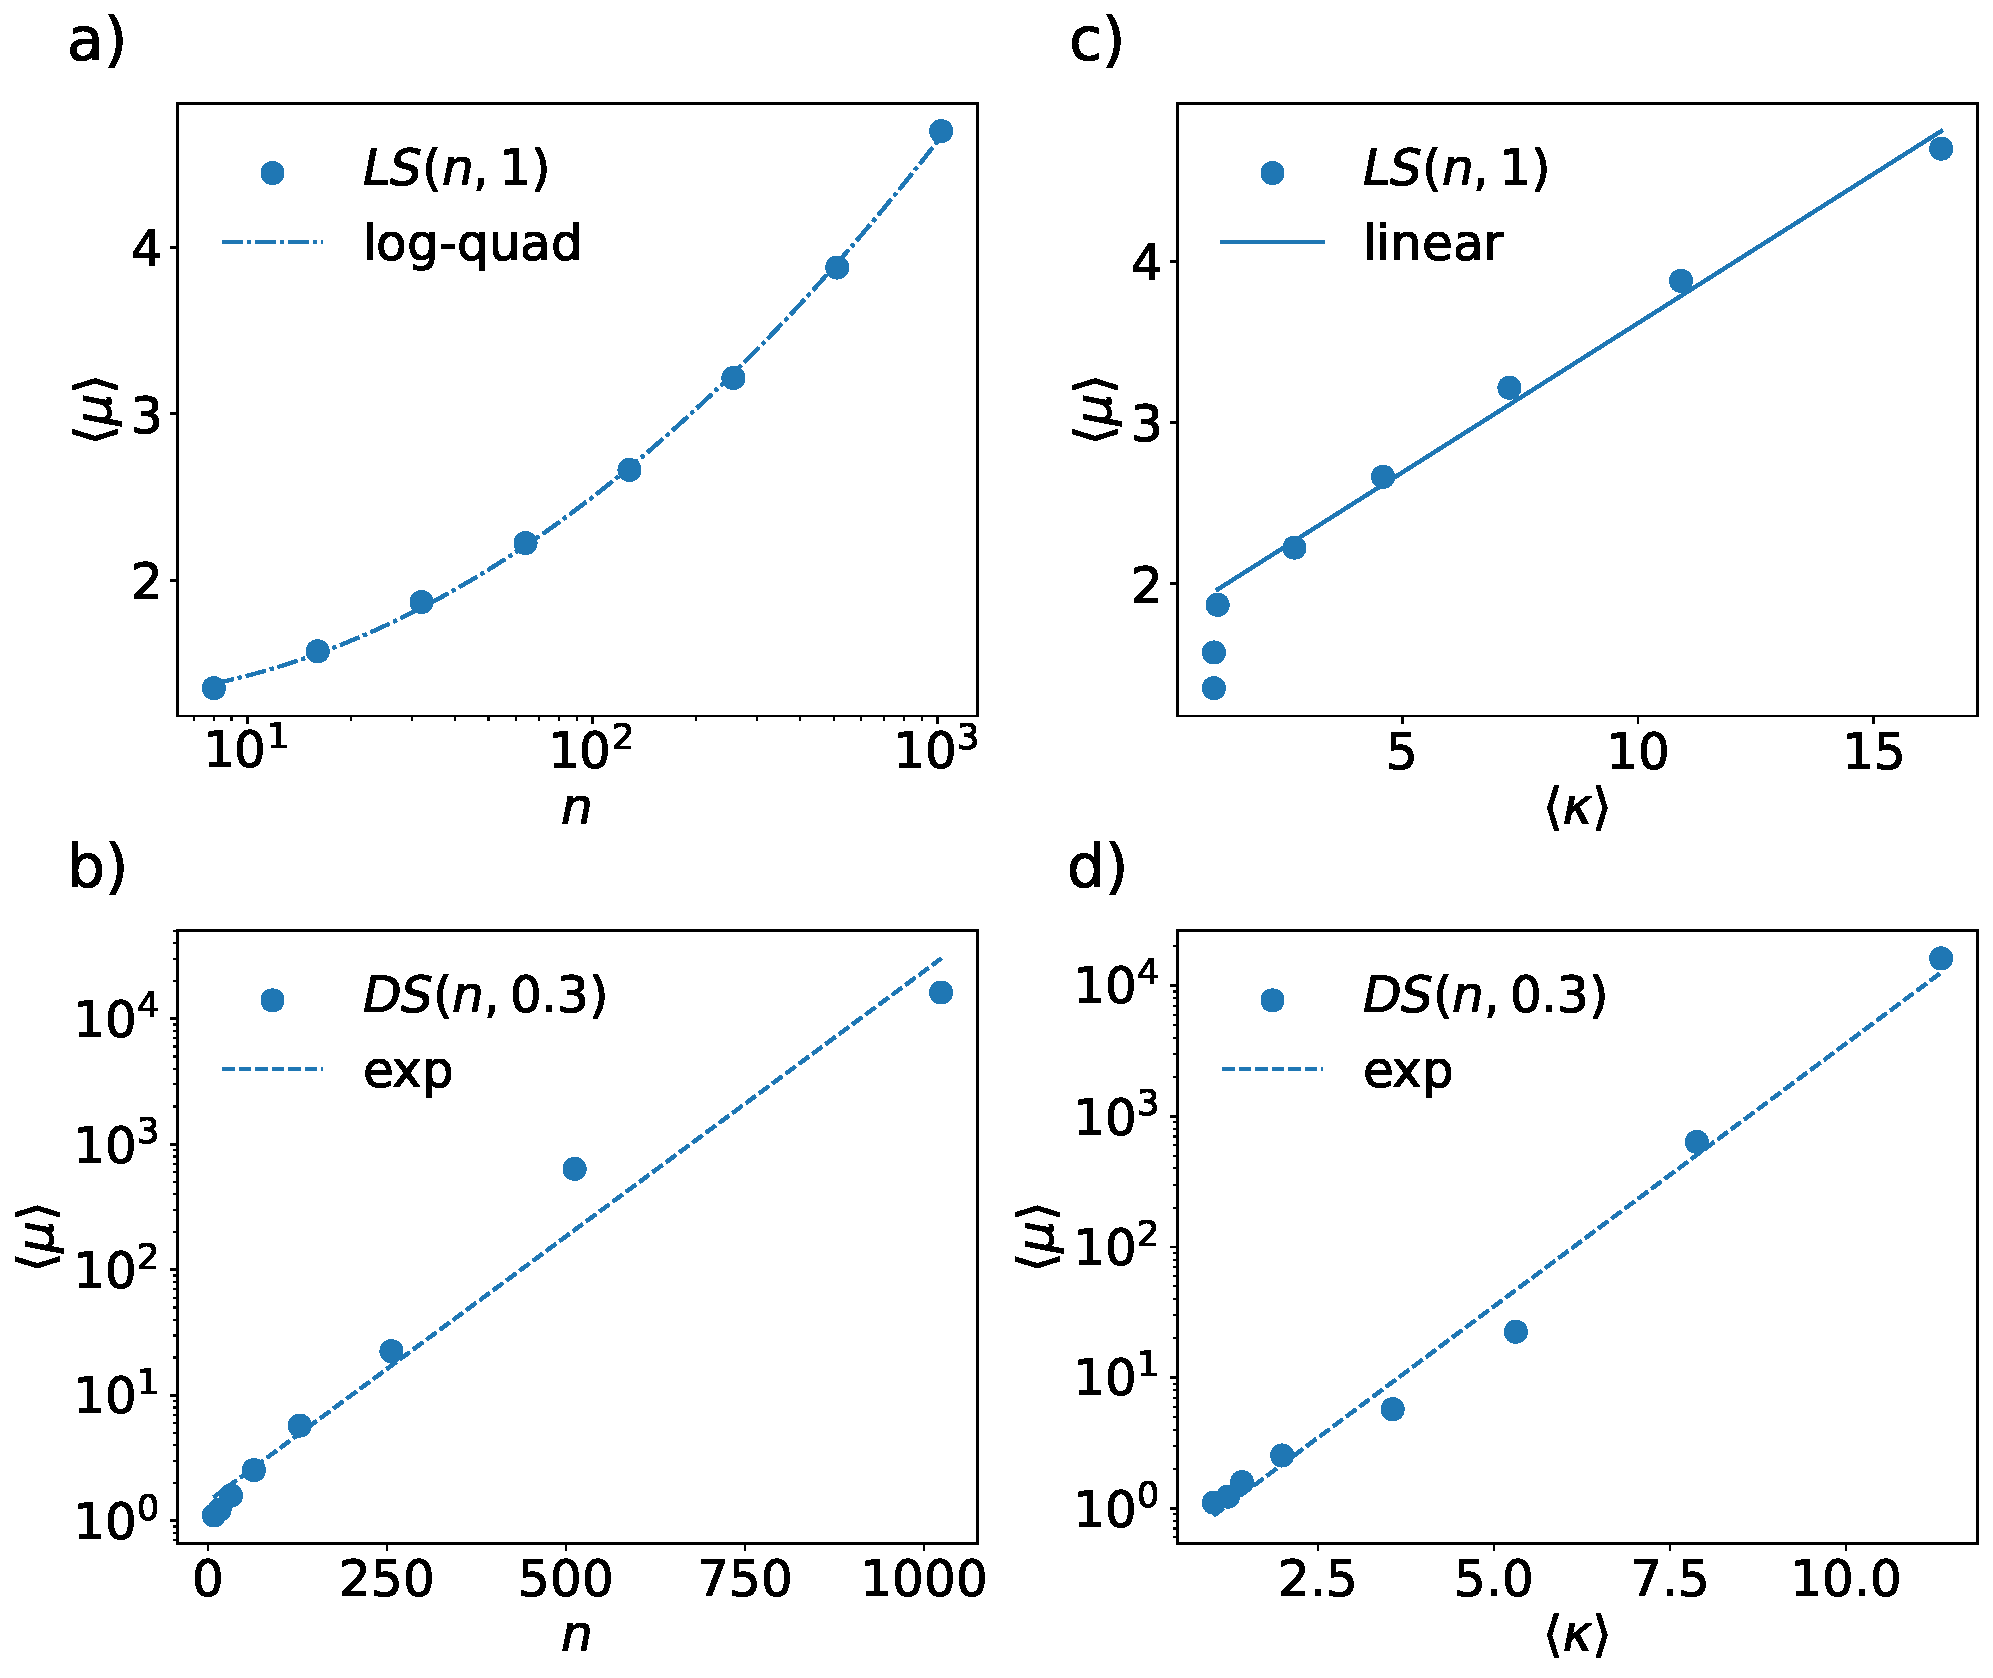
\includegraphics[width=3.4in]{fig2.pdf}
\caption{Scaling between the average shortest path multiplicity $\langle \mu\rangle$ and the network size $n$ for networks generated by the local-search and duplication-split local rules. The lines highlight the scaling specified in the legend. Note that it takes a critical network size $r_\kappa$ to detect network communities. Therefore, the scaling between $\langle\mu\rangle$ vs $\langle\kappa\rangle$ manifests for the largest network sizes simulated.}
\label{fig_local}
\end{figure}

\section{Networks with local structures}
\label{local}

Now we investigate the networks generated by the local rules, without rewiring. Although these local rules do not contain any pre-defined community structure, the resulting networks have communities as determined by standard methods of network communities detection  \cite{vazquez2025local}. In fact, beyond a certain network size $r_{\kappa}$, the Ramsey community number, the observation of network communities is almost certain. Now we proceed to uncover the scaling of the average shortest path multiplicity with the network size and with the number of inferred communities.

In all models investigated $\langle\mu\rangle$ is an increasing function of $n$. Furthermore, for all the network models with local rules the  average number of inferred communities $\langle\kappa\rangle$ increases with increasing $n$ as well. As a consequence, we can investigate the implicit relation between $\langle\mu\rangle$ and $\langle\kappa\rangle$.

Figure \ref{fig_local}a and b reports the data for the $LS(n, d=1)$ model: node addition, link creation to a randomly chosen existing node, local search stopping at 1 step, and link addition to the reached node. For this model $\langle\mu\rangle$ increases faster than linear with increasing $\log n$. A fit to the log-quadratic law
%
\begin{equation}
\langle\mu\rangle_{S,I} = a + b \log n + c (\log n)^2,
\label{mu_s1} 
\end{equation}
%
is consistent with the data points for the range of network sizes tested (Fig. \ref{fig_local}a, line). In turn, $\langle\mu\rangle$ exhibits a linear scaling with $\langle\kappa\rangle$ (Fig. \ref{fig_local}b).

Figure \ref{fig_local}c and d reports the data for the $DS(n, q=0.3)$ model: node addition and either node duplication with probability $q$, or link split otherwise. For this model $\langle\mu\rangle$ increases exponentially with $n$
%
\begin{equation}
\langle\mu\rangle_{S,II} = a e^{ b n},
\label{mu_s2} 
\end{equation}
%
where $a>0$ and $b>0$ (Fig. \ref{fig_local}c). $\langle\mu\rangle$ also exhibits an exponential scaling with $\langle\kappa\rangle$ (Fig. \ref{fig_local}d).

\begin{figure}
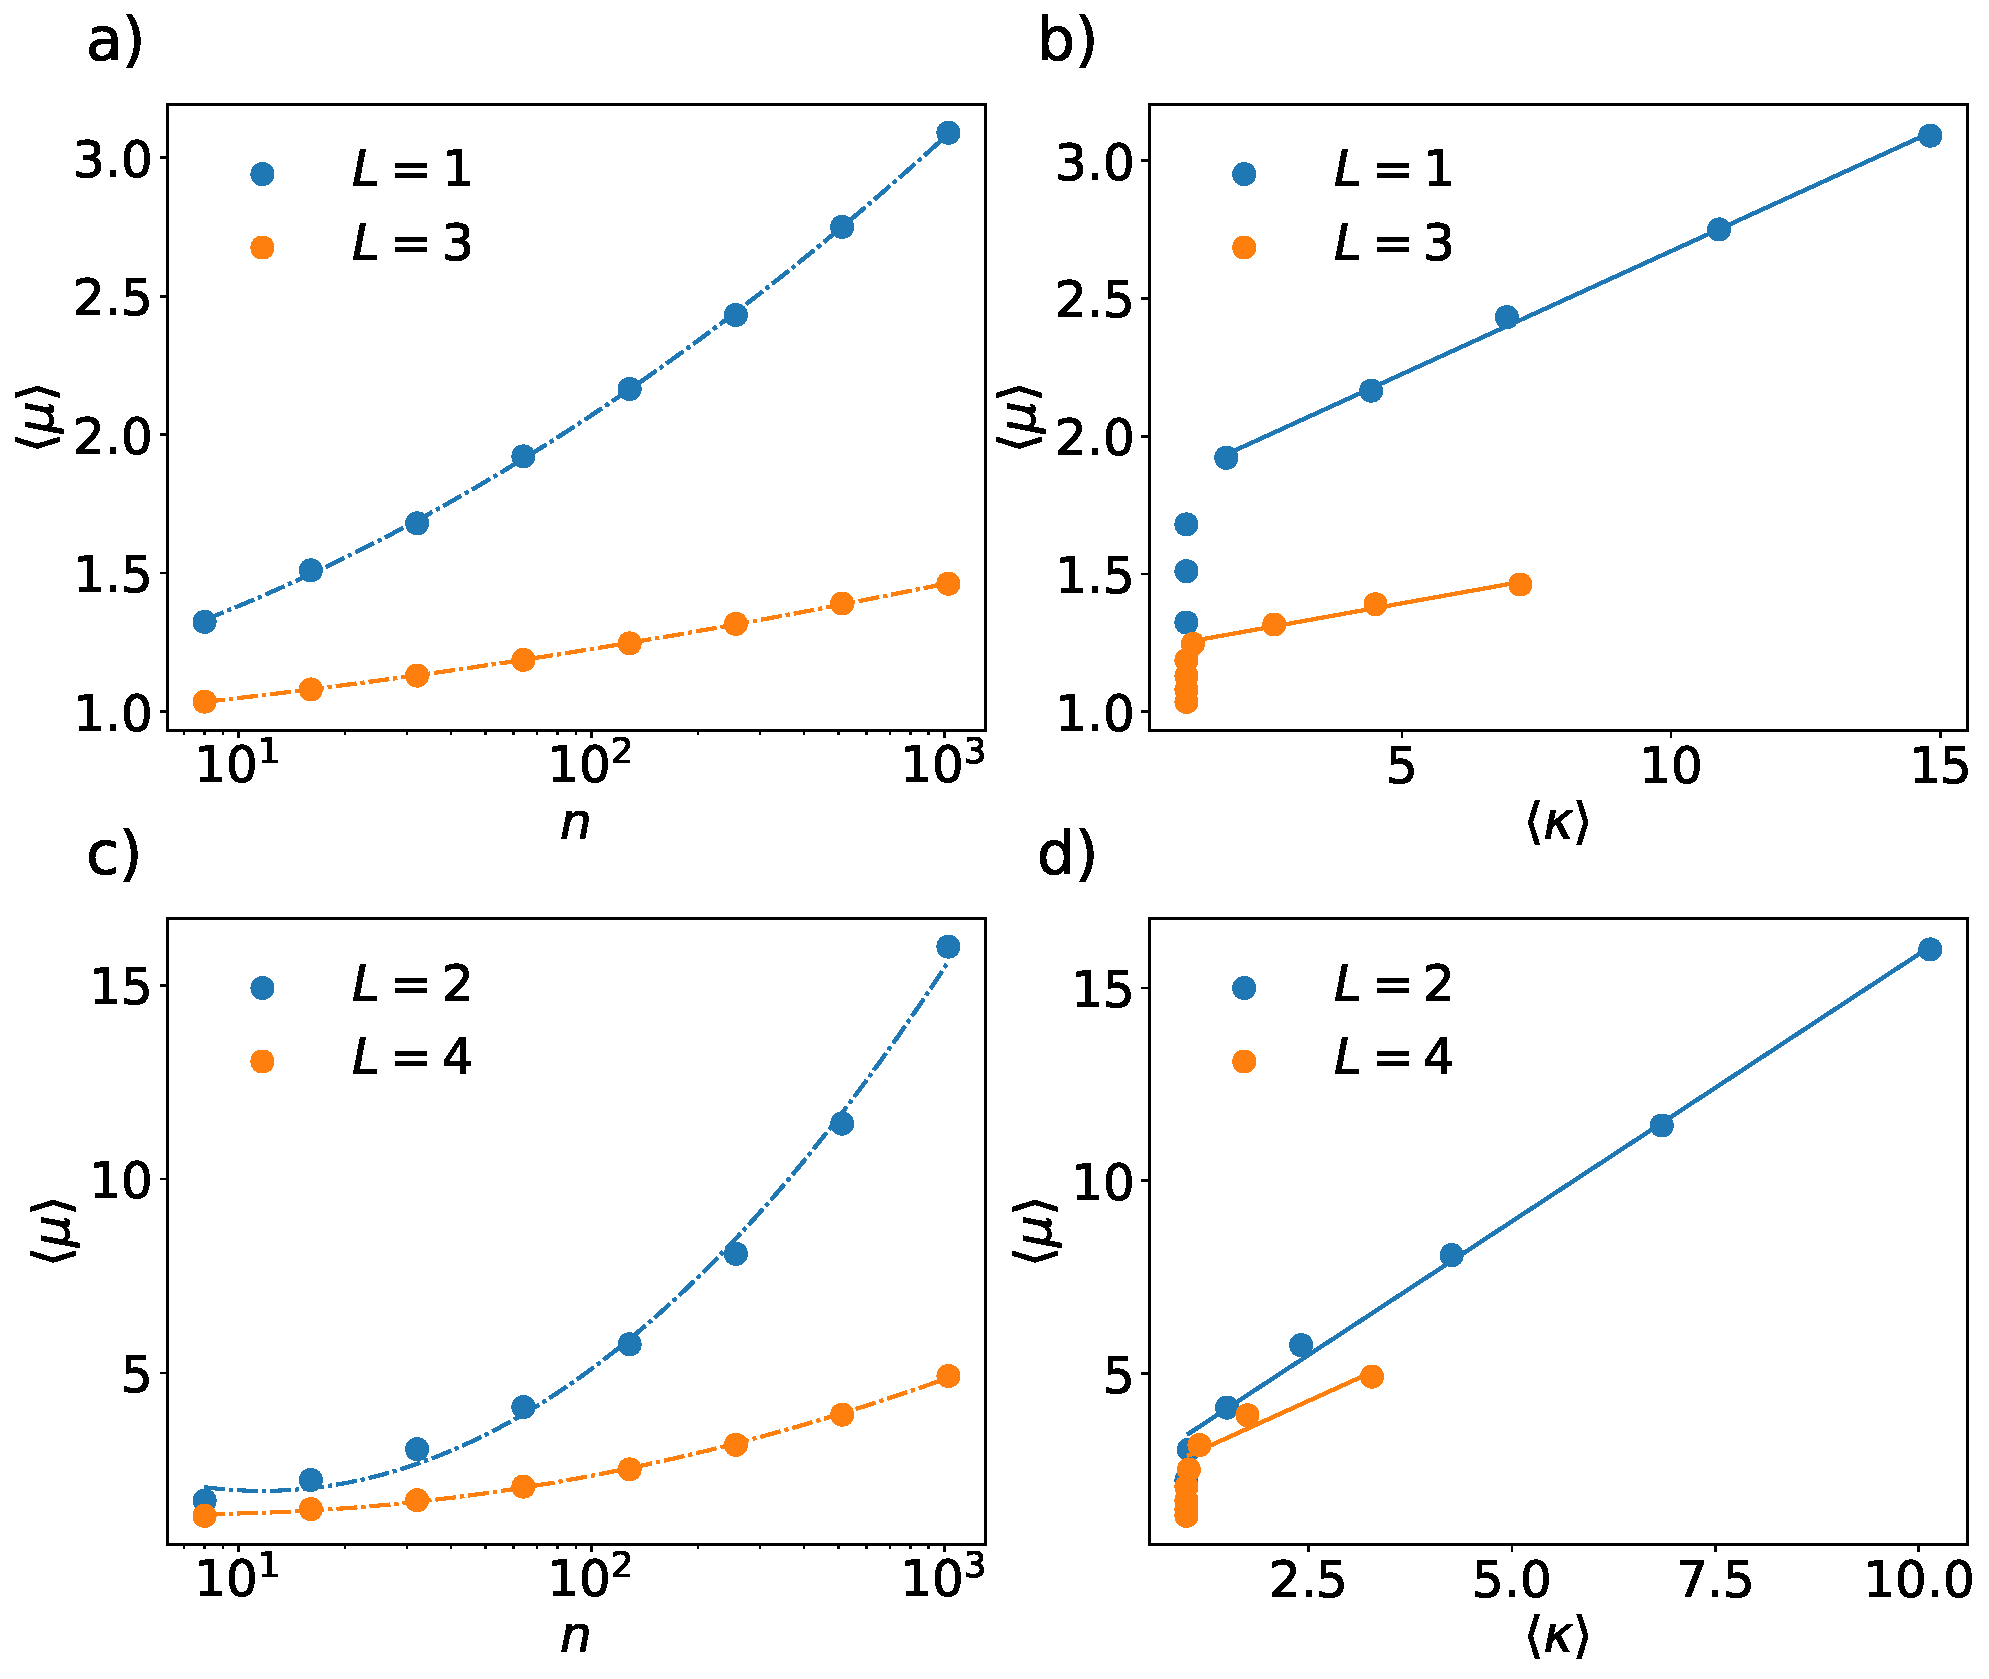
\includegraphics[width=3.4in]{fig3.pdf}
\caption{Scaling between the average shortest path multiplicity $\langle \mu\rangle$ and the network size $n$ for networks generated by the $BB(n, L)$ model. The lines highlight the scaling specified in the legend. Note that it takes a critical network size $r_\kappa$ to detect network communities. Therefore, the scaling between $\langle\mu\rangle$ vs $\langle\kappa\rangle$ manifests for the largest network sizes simulated.}
\label{fig_bubble}
\end{figure}

The differences between the local-search and duplication-split models could be related to the typical cycle length induced by the local rule. The triadic closure rule of $LS(n, 1)$ creates cycles of length 3. There is only one shortest path between the nodes in a 3-nodes cycle. In contrast, the duplication rule create cycles of length 4. Each node in a 4-cycle has two shortest paths to the opposite node two steps away. The duplication rule boosts the shortest path multiplicity. Note that this reasoning does not take into account the creation of multiple paths between existing nodes and passing through the new node, or between the new node and other existing nodes in the network. Such additional contribution is responsible for the type I scaling for the $LS(n, 1)$ networks.

The bubble model $BB(n, L)$ is a great tool to investigate the cycle length dependency. At each network update, a chain of $L$ nodes is connected to the ends of a randomly chosen link, thus forming a cycle of length $L+2$. For $L=2k-1$ with $k=1, 2,\ldots$ the bubble model generates cycles of odd length. Otherwise, for $L=2k$ with $k=1, 2,\ldots$  the cycles have even length. Based on the numerical simulations, $\langle\kappa\rangle$ reaches higher values for even $L$ than for odd $L$ (Fig. \ref{fig_bubble}). However, regardless of the $L$ parity, the scaling is log-quadratic, Eq. (\ref{mu_s1}) .

The exponential law Eq. (\ref{mu_s2}) should be rooted in some other aspect of the duplication rule. If the duplicated node has degree $k$ then it creates $k(k-1)/2$ squares. In turn there is preferential attachment. The link addition rate is $\pi_k = qk/n$. Using the rate equations for the nodes degree dynamics one obtains a power law degree distribution $p_k\sim k^{-\gamma}$ with $\gamma=1+1/q$. The average excess degree $\langle k(k-1)\rangle/2$ diverges with increasing $n$ for $q\geq 1/2$. Yet, we observe the exponential dependency in Eq. (\ref{mu_s2}) for $q=0.3$, where  $\langle k(k-1)\rangle/2$ is finite. The reason for the exponential scaling remains to be uncovered.

\begin{figure}
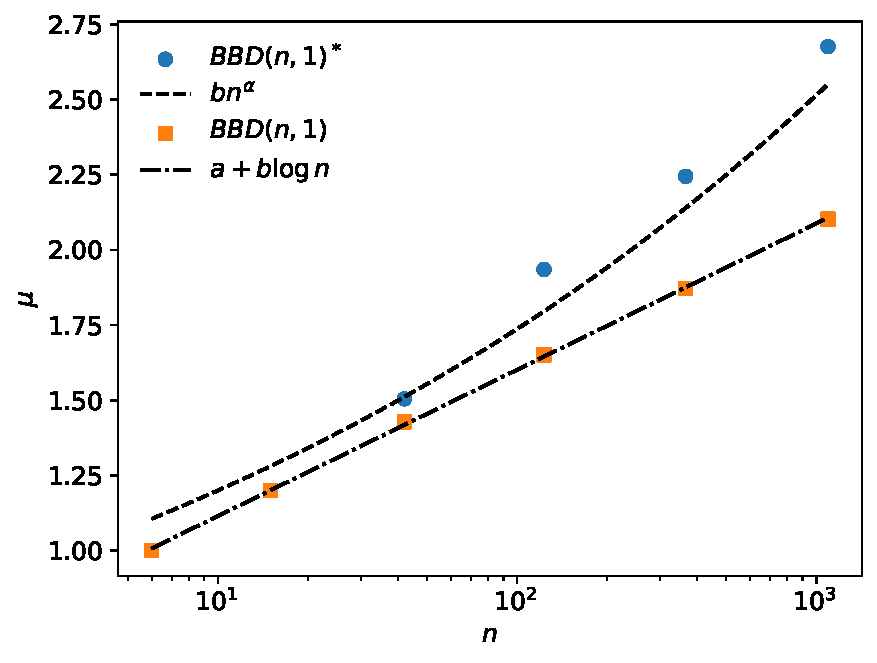
\includegraphics[width=3.4in]{fig4.pdf}
\caption{Scaling between the average shortest path multiplicity $\langle \mu\rangle$ and the network size $n$ for networks generated by the deterministic bubble model. The line highlights the log-linear scaling.}
\label{fig_deterministic}
\end{figure}

\section{Deterministic model}

Dorogovtsev, Goltsev and Mendes introduced a deterministic model for network growth with a recursive rule similar to the bubble model with $L=1$ \cite{dorogovtsev2002fractal}. The model is started at step $t=0$ with 3 connected nodes making a triangle. At each new step, new nodes are connected to both ends of every link in the current network. Given this deterministic recursion many properties can written down as a function of the step $t$ \cite{dorogovtsev2002fractal}.  I have attempted to derive a close expression between $\langle\mu\rangle$ and $n$, but I have failed. Surprisingly, the numerical results are better fitted by a log-linear relation, as observe for randomized networks (Fig. \ref{fig_deterministic}). This would suggest that the stochasticity of the local models plays some role in the observed log-quadratic scaling (Eq. \ref{mu_s1}). 

\section{Conclusions}
\label{conclusions}

In sparse networks without local structure, the average shortest path multiplicity $\langle\mu\rangle$ scales logarithmically with the network size $n$: $\langle\mu\rangle_{S,0} = a + b\log n$.

In sparse networks generated by local evolution rules,  we observe two types of scaling of the average shortest path multiplicity $\langle\mu\rangle$ vs $n$. For most models there is a log-quadratic scaling $\langle\mu\rangle_{S,I}= a + b\log n + c(\log n)^2$. In contrast, for the duplication-split model, a faster exponential growth $\langle\mu\rangle_{S,II} = a e^{bn}$ manifests.

Since the local evolution rules induce (i) the formation of network communities and (ii) the average number of communities $\langle\kappa\rangle$ increases with increasing the network size, then we can investigate the scaling between $\langle\mu\rangle$ and $\langle\kappa\rangle$. It is linear for all models tested, except for the duplication-split model where an exponential dependency was observed.

We could say local evolution rules and network communities are two sides of the same coin. With that view in mind, the statements that local evolution rules increase shortest path multiplicity and that network communities increase shortest path multiplicity  are equivalent. However, we should bear in mind that the local network evolution rules model the natural evolution of the systems they represent. In that regard, the local evolution rules are the driving mechanism and everything else follows.


\bibliographystyle{apsrev4-1}

%\bibliography{network.bib}

\documentclass[reprint,aps,pre,amsmath,amssymb,superscriptaddress,showpacs]{revtex4-1}
\usepackage{graphicx}
\usepackage{hyperref}
\usepackage{color}

\newtheorem{definition}{Definition}

\begin{document}

\title{Local network evolution rules drive shortest path multiplicity}

\author{Alexei Vazquez}
\email{alexei@nodeslinks.com}
\affiliation{Nodes \& Links Ltd, Salisbury House, Station Road, Cambridge, CB1 2LA, UK}

\begin{abstract}
The shortest path multiplicity is an important metric of complex networks. The shortest path multiplicity of real networks is high and it correlates with their community structure. Since local network evolution induces network communities, it is possible that a high shortest path multiplicity is the natural expectation of local evolution rules. Here I demonstrate, by means of numerical simulations, that this is indeed the case.
\end{abstract}

\maketitle

\section{Introduction}

The fundamental question of network science is to determine the minimum set of properties and models to explain what we observe in real networks. New discoveries should be subject to the scrutiny of existing concepts. That is the case of the  recent observation by Deng {\em et al} \cite{deng2026multipath}, a correlation between the number of communities and the density of multiple shortest paths in real networks. This correlation could be the consequence of an upstream factor that causes both features. And it turns out that there is an obvious candidate: local evolution rules.

Local network evolution rules are node/link addition mechanisms of network growth \cite{vazquez03local}. Local rules are inspired by the natural evolution of real networks. Web pages are created by copying other pages \cite{kleinberg99}. We cite references that we found reading another publication \cite{vazquez01rs}. Friends of friends become friends \cite{growing_social_networks_jin01}.  Proteins increase their connectivity when their interacting partners are duplicated \cite{vazquez03dup, pastor-satorras03}. Local evolution rules lead to the emergence of network communities: beyond a certain network size we can warrant that the network will exhibit communities \cite{vazquez2025local}. These communities are not written in the network evolution rules. Yet they are imputed by the state of the art methods to detect network communities.

Local evolution rules induce the formation of short cycles and cycles tend to increase the shortest path multiplicity. Therefore, I raise the hypothesis that the high shortest path multiplicity of real networks is rooted on their local growth dynamics. Furthermore, since those local rules induce the formation of networks communities, that would explain the association between shortest path multiplicity and network communities as well.

In this work I investigate this hypothesis by means of numerical simulations. In the Sec. \ref{methods} I introduce different models of growing networks with local rules and the methods used to quantify their properties. In Sec. \ref{random} I characterize random networks without local structures to set the baseline expectation. In Sec. \ref{local} I characterize the networks generated by local rules. The concluding remarks are reported in Sec. \ref{conclusions}.

\section{Methods}
\label{methods}

The computer code related to these methods is available at \href{https://github.com/av2atgh/ramsey_netcom}{github.com/av2atgh/ramsey\_netcom}.

\subsection{Local models}

Local search $LS(n, d)$. {\em Initial condition}. The network is started with two connected nodes. Evolution rule: A new node is added and a $d$-step random walk is performed from a randomly selected node in the current network. The new node is connected to all
visited nodes. This model has preferential attachment because the probability that a node is visited, beyond the entry node, is proportional to the current nodes degrees. Consequently it generate networks with a power law degree distribution. The $LS(n, d)$ networks have a
high clustering coefficient. At least 1 triangle, between the entry point and next neighbor visited, is formed at every node addition. For $d=1$ this model is equivalent to the triadic closure model \cite{growing_social_networks_jin01, communities_bianconi_2014}.

Duplication split $DS(n, q)$. {\em Initial condition}: The network is started with two connected nodes. {\em Evolution rule}: A new node $i$ is added to the network and a node in the current network is selected at random, node $j$. With probability $q$, $i$ becomes a duplicate of $j$ with links from $i$ to all neighbors of $j$. Otherwise, a link between $j$ and a randomly selected neighbor of $j$, node $k$, is split. The edge $(j, k)$ is removed and new edges $(i, j)$ and $(i, k)$ are created. This model has preferential attachment because, for the duplication rule, the probability that a node neighbor is duplicated is proportional to the node degree. The duplication rule does not make triangles and the split rule breaks triangles if they would exist. The main motif of this model is the formation of squares (cycles of length 4) between any two neighbors of the reference node $j$ and its duplicate $i$.

Bubble model $BB(n, L)$. {\em Initial condition}: The network is started with two connected nodes. {\em Evolution rule}: A chain of $L$ new nodes is added to the network. The two nodes at the chain ends are attached to the ends of an existing link, creating a cycle of length $L+2$. $BB(n, 1)$ is equivalent to an earlier Dorogovtsev-Mendes model where new nodes are connected to both ends of a randomly chosen link by two undirected links \cite{dorogotsev2001link}. The model has preferential attachment because the probability that a node is at the end of the selected link is proportional to its degree. The main network motif are the cycles of length $L+2$ created by the evolution rule.

All these models have a finite Ramsey community number $r_\kappa$, the minimum graph size that guarantees the emergence of network communities with almost certainty \cite{vazquez2025local}.

\subsection{Network communities}

The network communities are inferred using the stochastic block model implemented in graph-tool (\verb|graph_tool.inference.minimize_blockmodel_dl|, with default parameters) \cite{peixoto_graph-tool_2014}. This stochastic block model finds the community structure with the minimum description length \cite{peixoto2024networkreconstructionminimumdescription}. In that sense, it gives as output the optimal number of communities $\kappa$ and the partition of the nodes into communities. The average of $\kappa$ is calculated from 100 realizations of network creation plus network community inference.

An important parameter is the correction for the network degree sequence, \verb| deg_corr: bool (optional, default: True)|. Some of the networks investigated have power law degree distributions, and therefore I use the degree-corrected version of the stochastic block model (default option). Similar results are obtained using the Infomap method implemented in the package with the same name \cite{mapequation2025software}, as previously shown \cite{vazquez2025local}.

\subsection{Network rewiring}

For network rewiring, I use the standard configuration model implemented with \verb|graph_tool.generation.random_rewire| with default parameters. The configuration algorithm rewires the network links preserving the degree distribution \cite{configuration_method_park_2004}.

\subsection{Shortest path multiplicity}

To determine the path multiplicity $\mu_{ij}(G)$ between a pair of nodes $(i, j)$ in graph $G$, I use the graph-tool method \verb|graph_tool.count_shortest_paths(G, i, j)| with default parameters.

Given a graph generator $f_G$, I calculate the average shortest path multiplicity $\langle \mu\rangle$ as the average over every pair of nodes and over 100 realizations of $G$.

\begin{figure}
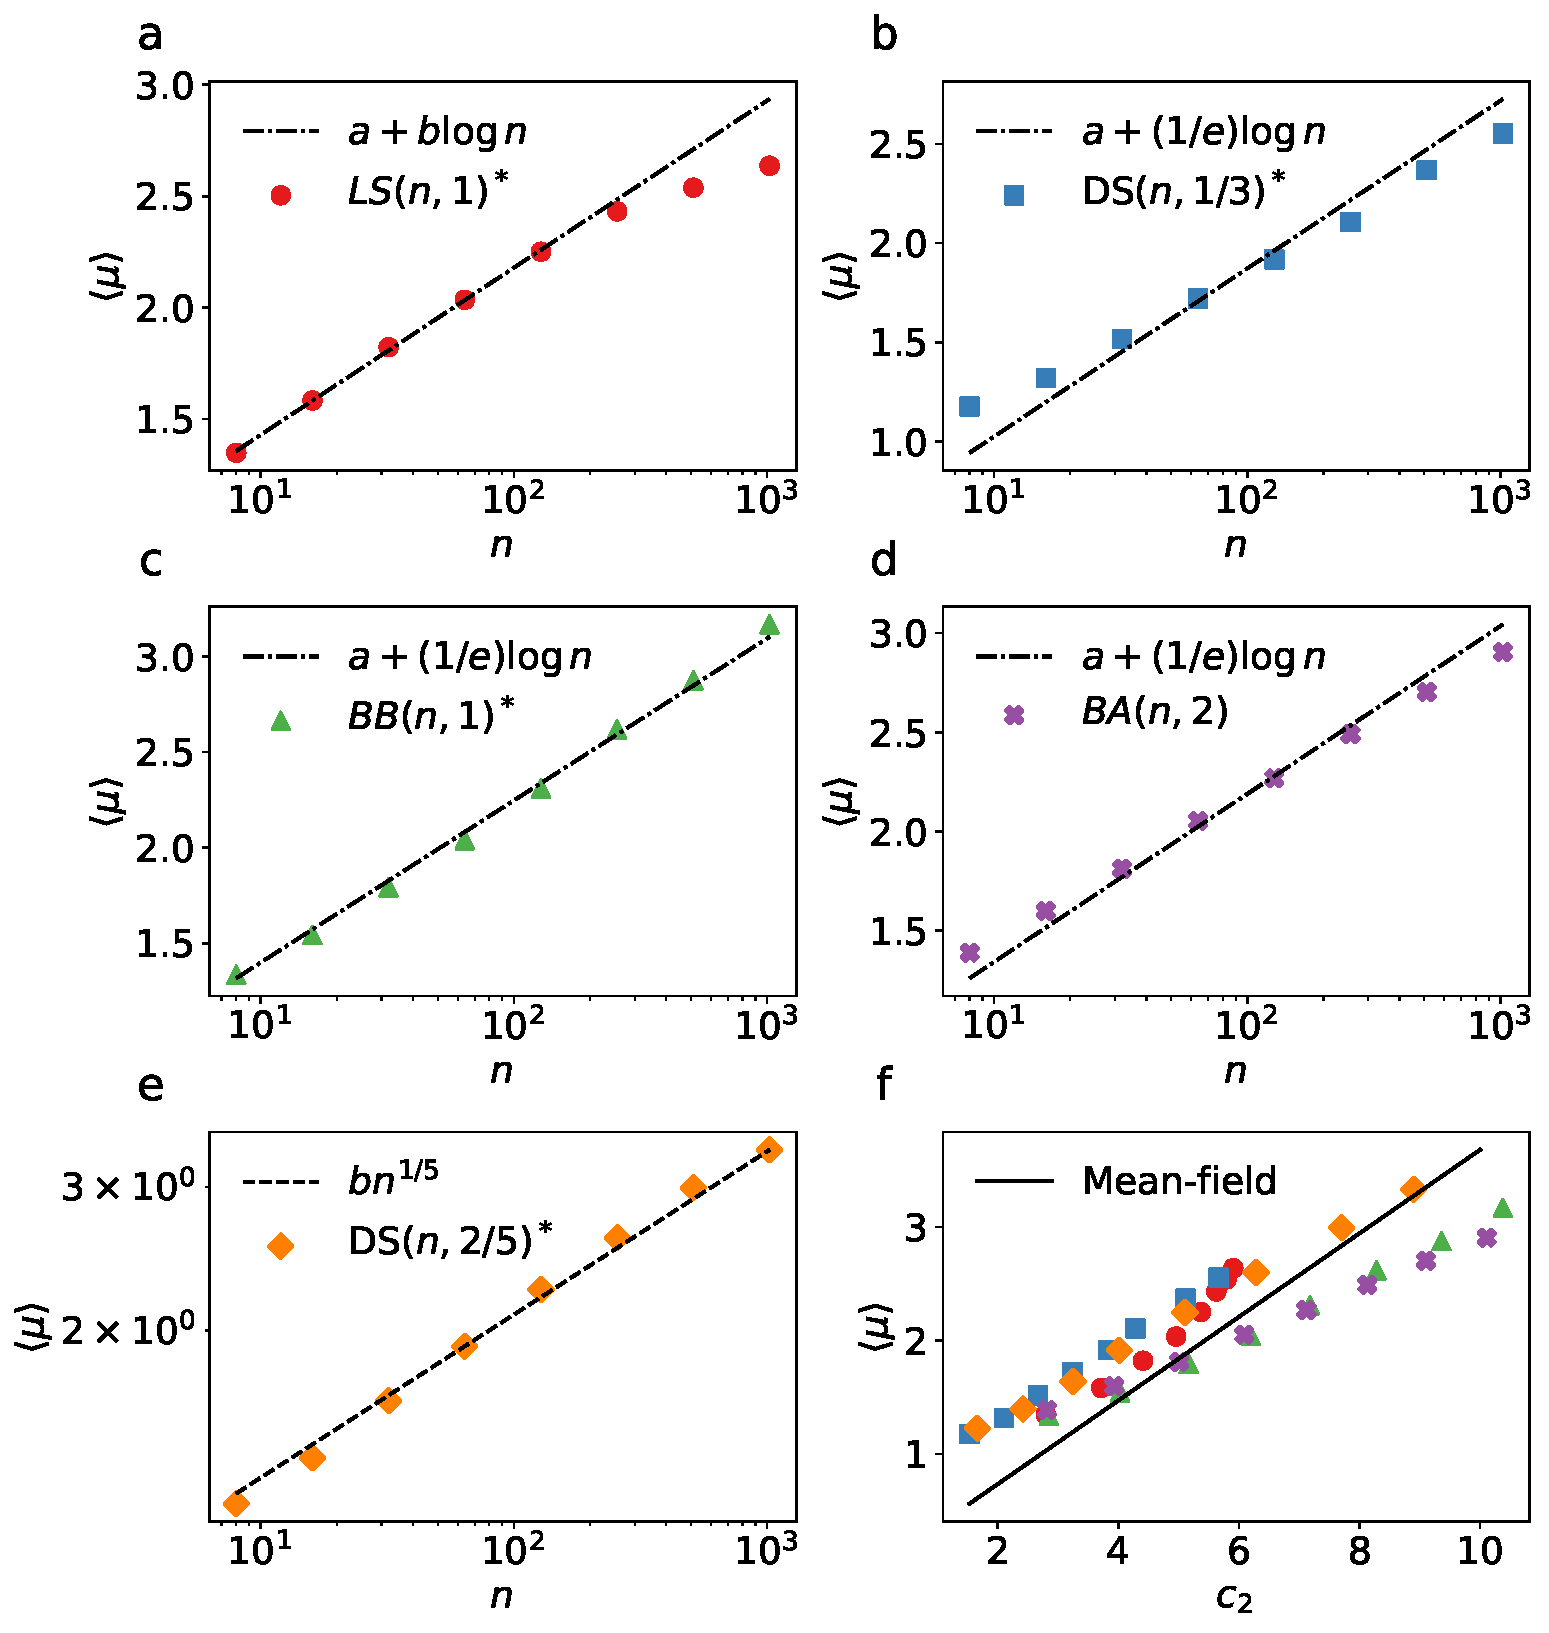
\includegraphics[width=3.4in]{fig1.pdf}
\caption{Scaling between the average shortest path multiplicity $\langle \mu\rangle$ and the network size $n$ for randomized networks. The networks were generated using the local rule indicated in the legend and then randomized by the degree preserving link rewiring. The lines highlight the logarithmic scaling.}
\label{fig_randomized}
\end{figure}

\section{Non-structured networks}
\label{random}

Dong {\em et al} \cite{dong2025multi} have estimated the network size scaling of the average shortest path multiplicity  for the Erd\"os-R\'enyi random graph model $ER(n, p)$, denoted by $\langle \mu\rangle_{ER}$. In the dense regime, $p$ near and above 0.1, $\langle \mu\rangle_{ER}$ scales linearly with $n$. However, real networks are sparse, corresponding to $p\sim1/n$.

To investigate sparse random networks, we can use as starting point the local rule models and then we apply the degree preserving link rewiring method. Figure \ref{fig_randomized} shows the average shortest path multiplicity $\langle \mu\rangle$ as a function of the network size $n$, the number of nodes. For all the sparse random networks tested there is a logarithmic growth
%
\begin{equation}
\langle \mu\rangle_{S,0} = a + b\log n,
\label{mu_rnd} 
\end{equation}
%
as it is emphasized by the fitted line in the semi-log plot. That is indeed slower than the linear dependency for the Erd\"os-R\'enyi graphs in the dense regime. The subscript {S0} stands for sparse network (S) and non-structured network (0). 

\begin{figure}
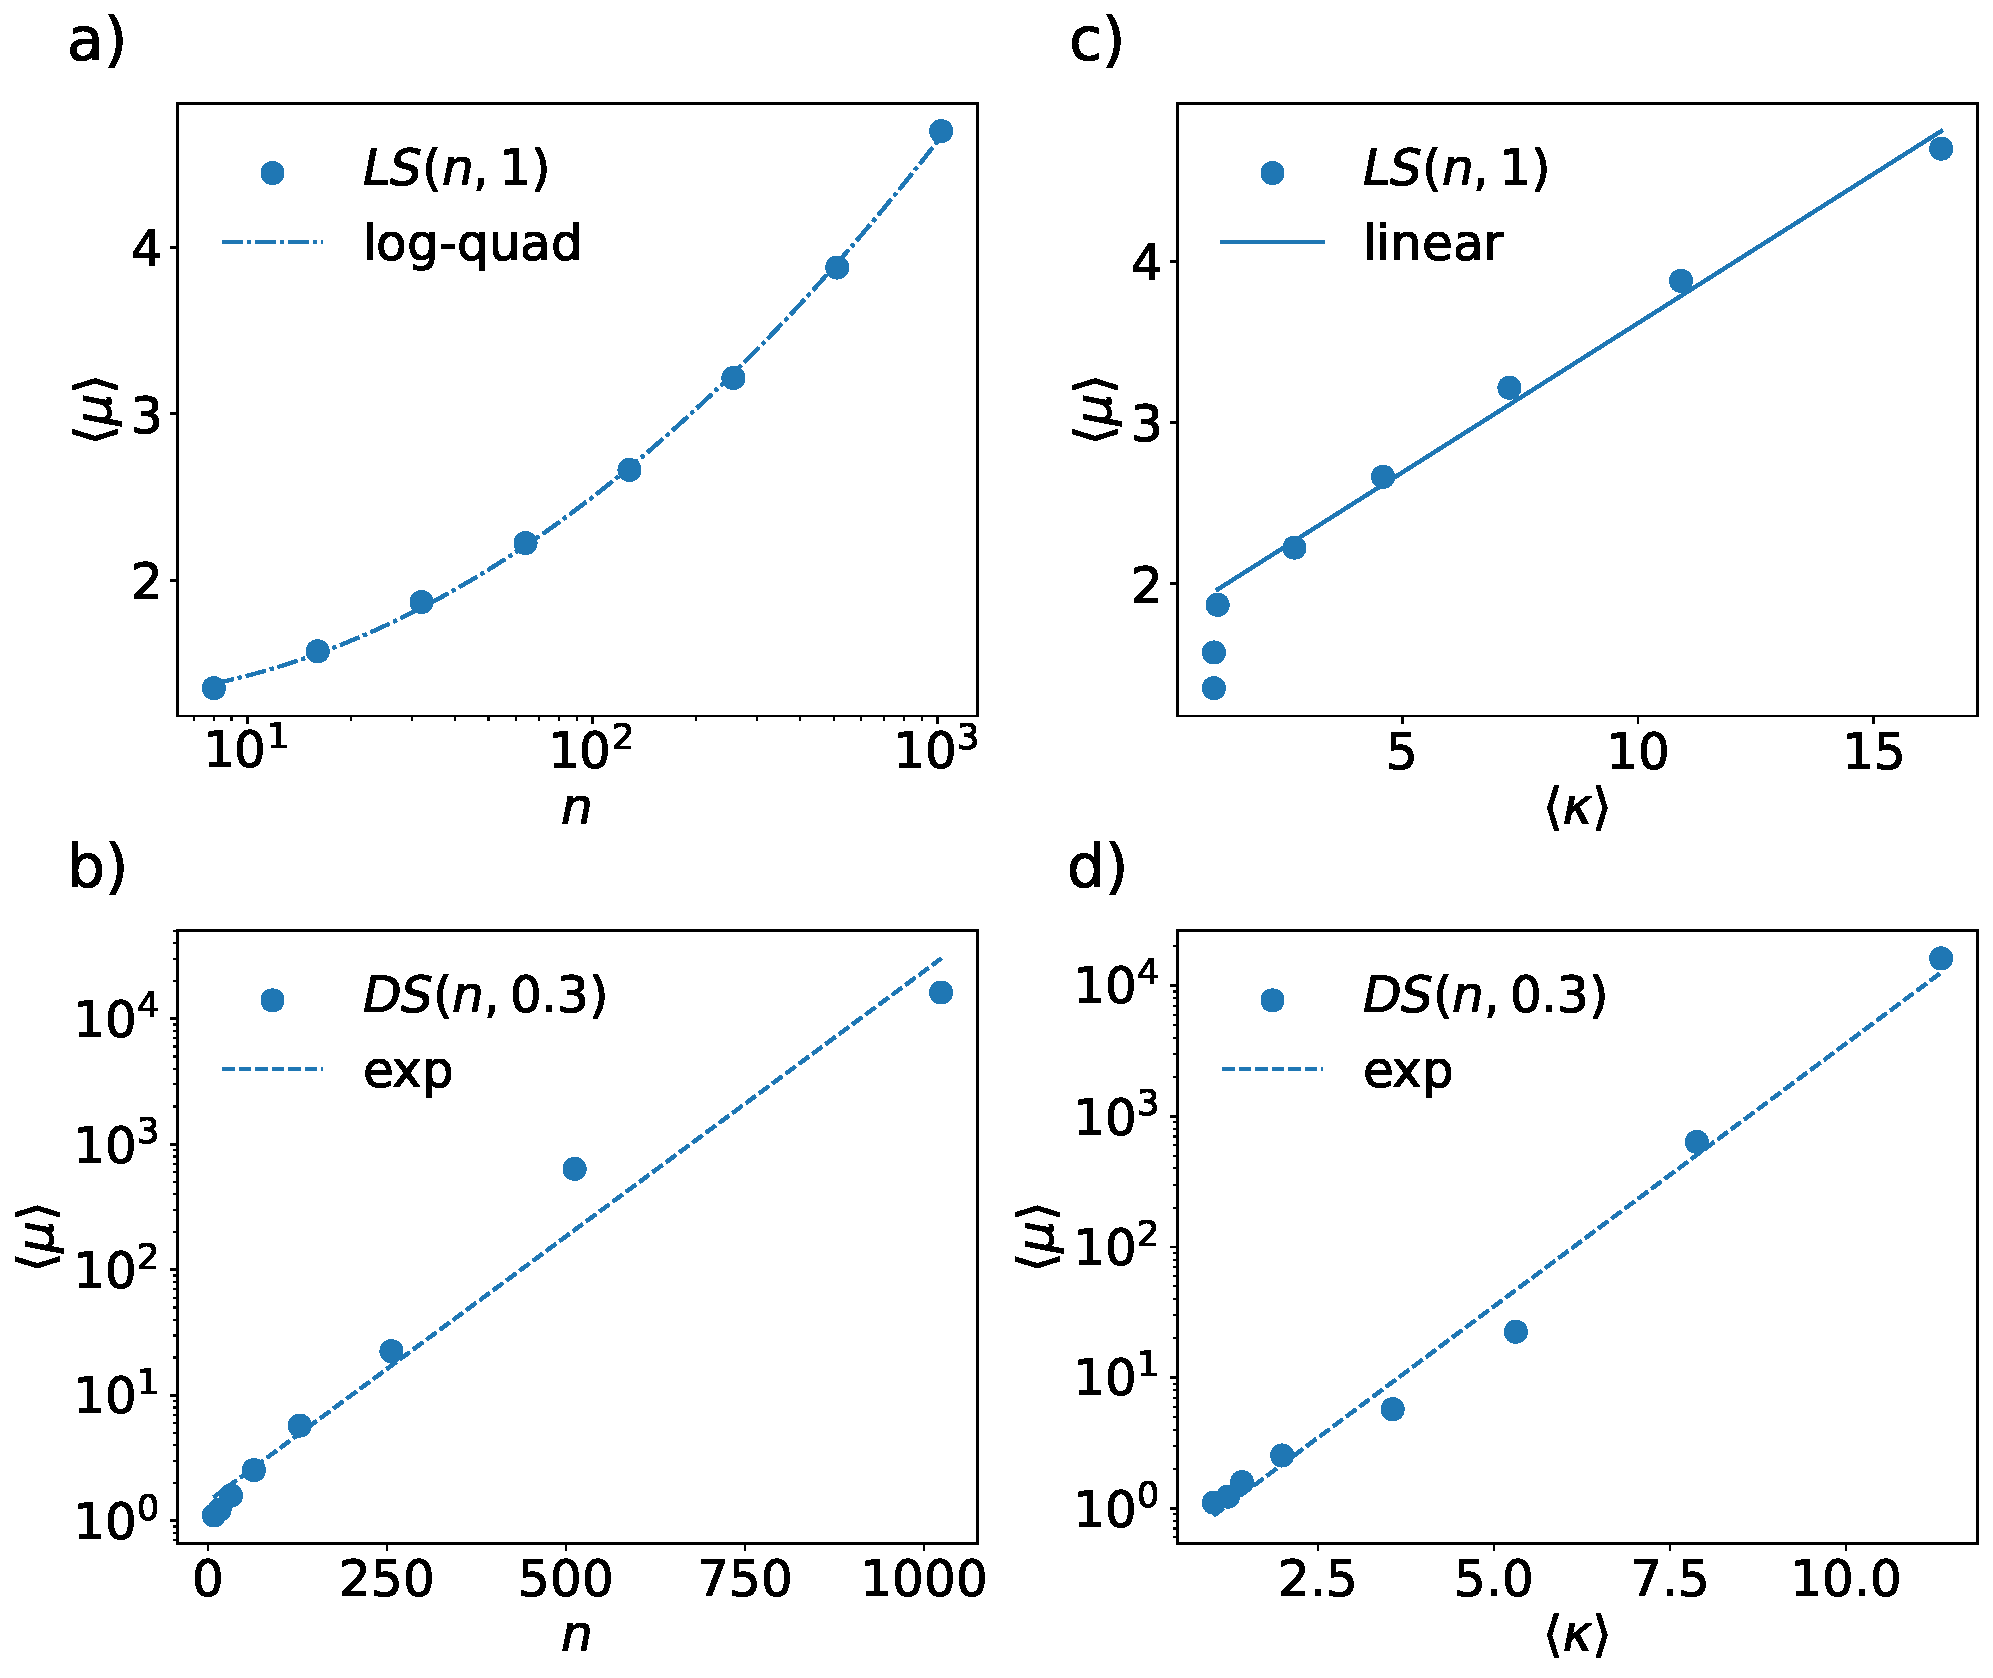
\includegraphics[width=3.4in]{fig2.pdf}
\caption{Scaling between the average shortest path multiplicity $\langle \mu\rangle$ and the network size $n$ for networks generated by the local-search and duplication-split local rules. The lines highlight the scaling specified in the legend. Note that it takes a critical network size $r_\kappa$ to detect network communities. Therefore, the scaling between $\langle\mu\rangle$ vs $\langle\kappa\rangle$ manifests for the largest network sizes simulated.}
\label{fig_local}
\end{figure}

\section{Networks with local structures}
\label{local}

Now we investigate the networks generated by the local rules, without rewiring. Although these local rules do not contain any pre-defined community structure, the resulting networks have communities as determined by standard methods of network communities detection  \cite{vazquez2025local}. In fact, beyond a certain network size $r_{\kappa}$, the Ramsey community number, the observation of network communities is almost certain. Now we proceed to uncover the scaling of the average shortest path multiplicity with the network size and with the number of inferred communities.

In all models investigated $\langle\mu\rangle$ is an increasing function of $n$. Furthermore, for all the network models with local rules the  average number of inferred communities $\langle\kappa\rangle$ increases with increasing $n$ as well. As a consequence, we can investigate the implicit relation between $\langle\mu\rangle$ and $\langle\kappa\rangle$.

Figure \ref{fig_local}a and b reports the data for the $LS(n, d=1)$ model: node addition, link creation to a randomly chosen existing node, local search stopping at 1 step, and link addition to the reached node. For this model $\langle\mu\rangle$ increases faster than linear with increasing $\log n$. A fit to the log-quadratic law
%
\begin{equation}
\langle\mu\rangle_{S,I} = a + b \log n + c (\log n)^2,
\label{mu_s1} 
\end{equation}
%
is consistent with the data points for the range of network sizes tested (Fig. \ref{fig_local}a, line). In turn, $\langle\mu\rangle$ exhibits a linear scaling with $\langle\kappa\rangle$ (Fig. \ref{fig_local}b).

Figure \ref{fig_local}c and d reports the data for the $DS(n, q=0.3)$ model: node addition and either node duplication with probability $q$, or link split otherwise. For this model $\langle\mu\rangle$ increases exponentially with $n$
%
\begin{equation}
\langle\mu\rangle_{S,II} = a e^{ b n},
\label{mu_s2} 
\end{equation}
%
where $a>0$ and $b>0$ (Fig. \ref{fig_local}c). $\langle\mu\rangle$ also exhibits an exponential scaling with $\langle\kappa\rangle$ (Fig. \ref{fig_local}d).

\begin{figure}
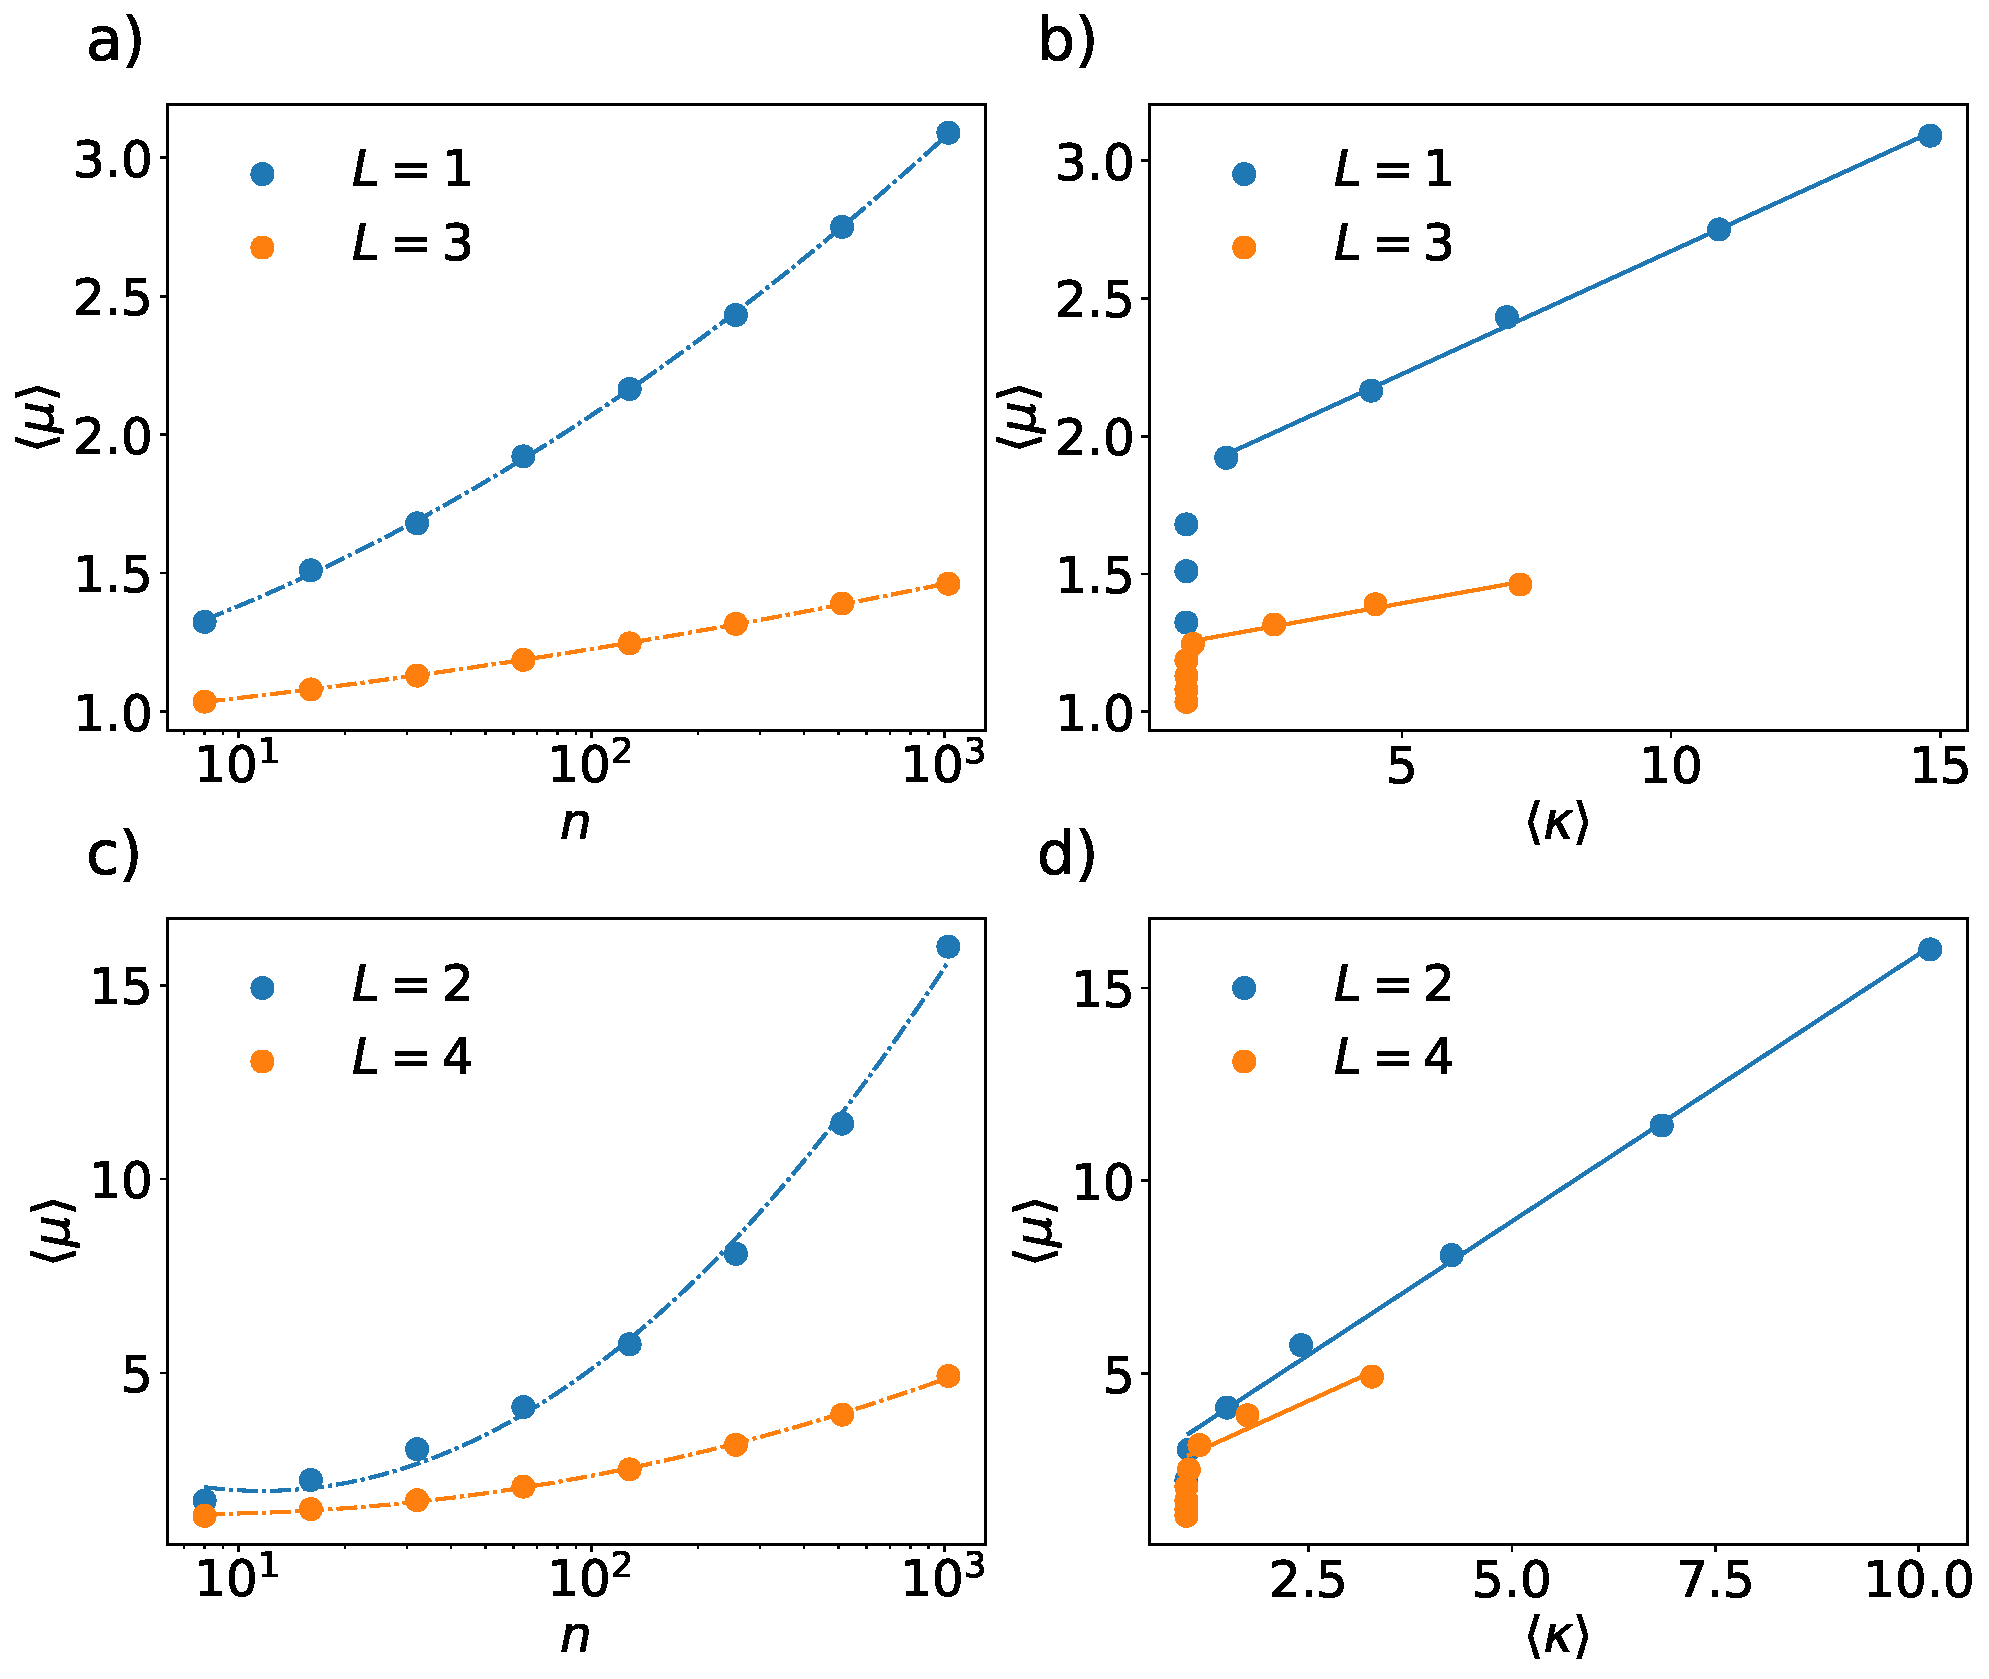
\includegraphics[width=3.4in]{fig3.pdf}
\caption{Scaling between the average shortest path multiplicity $\langle \mu\rangle$ and the network size $n$ for networks generated by the $BB(n, L)$ model. The lines highlight the scaling specified in the legend. Note that it takes a critical network size $r_\kappa$ to detect network communities. Therefore, the scaling between $\langle\mu\rangle$ vs $\langle\kappa\rangle$ manifests for the largest network sizes simulated.}
\label{fig_bubble}
\end{figure}

The differences between the local-search and duplication-split models could be related to the typical cycle length induced by the local rule. The triadic closure rule of $LS(n, 1)$ creates cycles of length 3. There is only one shortest path between the nodes in a 3-nodes cycle. In contrast, the duplication rule create cycles of length 4. Each node in a 4-cycle has two shortest paths to the opposite node two steps away. The duplication rule boosts the shortest path multiplicity. Note that this reasoning does not take into account the creation of multiple paths between existing nodes and passing through the new node, or between the new node and other existing nodes in the network. Such additional contribution is responsible for the type I scaling for the $LS(n, 1)$ networks.

The bubble model $BB(n, L)$ is a great tool to investigate the cycle length dependency. At each network update, a chain of $L$ nodes is connected to the ends of a randomly chosen link, thus forming a cycle of length $L+2$. For $L=2k-1$ with $k=1, 2,\ldots$ the bubble model generates cycles of odd length. Otherwise, for $L=2k$ with $k=1, 2,\ldots$  the cycles have even length. Based on the numerical simulations, $\langle\kappa\rangle$ reaches higher values for even $L$ than for odd $L$ (Fig. \ref{fig_bubble}). However, regardless of the $L$ parity, the scaling is log-quadratic, Eq. (\ref{mu_s1}) .

The exponential law Eq. (\ref{mu_s2}) should be rooted in some other aspect of the duplication rule. If the duplicated node has degree $k$ then it creates $k(k-1)/2$ squares. In turn there is preferential attachment. The link addition rate is $\pi_k = qk/n$. Using the rate equations for the nodes degree dynamics one obtains a power law degree distribution $p_k\sim k^{-\gamma}$ with $\gamma=1+1/q$. The average excess degree $\langle k(k-1)\rangle/2$ diverges with increasing $n$ for $q\geq 1/2$. Yet, we observe the exponential dependency in Eq. (\ref{mu_s2}) for $q=0.3$, where  $\langle k(k-1)\rangle/2$ is finite. The reason for the exponential scaling remains to be uncovered.

\begin{figure}
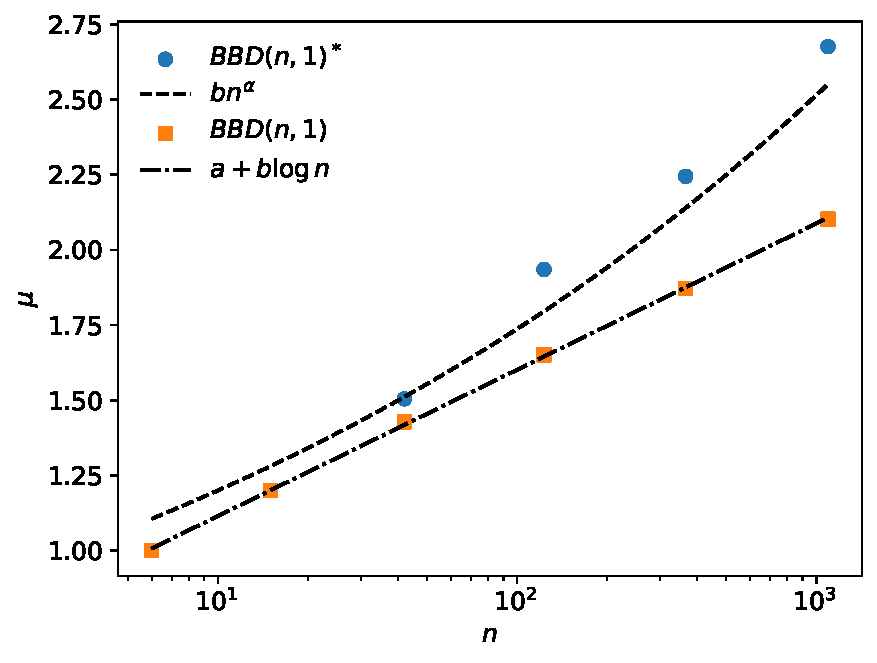
\includegraphics[width=3.4in]{fig4.pdf}
\caption{Scaling between the average shortest path multiplicity $\langle \mu\rangle$ and the network size $n$ for networks generated by the deterministic bubble model. The line highlights the log-linear scaling.}
\label{fig_deterministic}
\end{figure}

\section{Deterministic model}

Dorogovtsev, Goltsev and Mendes introduced a deterministic model for network growth with a recursive rule similar to the bubble model with $L=1$ \cite{dorogovtsev2002fractal}. The model is started at step $t=0$ with 3 connected nodes making a triangle. At each new step, new nodes are connected to both ends of every link in the current network. Given this deterministic recursion many properties can written down as a function of the step $t$ \cite{dorogovtsev2002fractal}.  I have attempted to derive a close expression between $\langle\mu\rangle$ and $n$, but I have failed. Surprisingly, the numerical results are better fitted by a log-linear relation, as observe for randomized networks (Fig. \ref{fig_deterministic}). This would suggest that the stochasticity of the local models plays some role in the observed log-quadratic scaling (Eq. \ref{mu_s1}). 

\section{Conclusions}
\label{conclusions}

In sparse networks without local structure, the average shortest path multiplicity $\langle\mu\rangle$ scales logarithmically with the network size $n$: $\langle\mu\rangle_{S,0} = a + b\log n$.

In sparse networks generated by local evolution rules,  we observe two types of scaling of the average shortest path multiplicity $\langle\mu\rangle$ vs $n$. For most models there is a log-quadratic scaling $\langle\mu\rangle_{S,I}= a + b\log n + c(\log n)^2$. In contrast, for the duplication-split model, a faster exponential growth $\langle\mu\rangle_{S,II} = a e^{bn}$ manifests.

Since the local evolution rules induce (i) the formation of network communities and (ii) the average number of communities $\langle\kappa\rangle$ increases with increasing the network size, then we can investigate the scaling between $\langle\mu\rangle$ and $\langle\kappa\rangle$. It is linear for all models tested, except for the duplication-split model where an exponential dependency was observed.

We could say local evolution rules and network communities are two sides of the same coin. With that view in mind, the statements that local evolution rules increase shortest path multiplicity and that network communities increase shortest path multiplicity  are equivalent. However, we should bear in mind that the local network evolution rules model the natural evolution of the systems they represent. In that regard, the local evolution rules are the driving mechanism and everything else follows.


\bibliographystyle{apsrev4-1}

%\bibliography{network.bib}

\documentclass[reprint,aps,pre,amsmath,amssymb,superscriptaddress,showpacs]{revtex4-1}
\usepackage{graphicx}
\usepackage{hyperref}
\usepackage{color}

\newtheorem{definition}{Definition}

\begin{document}

\title{Local network evolution rules drive shortest path multiplicity}

\author{Alexei Vazquez}
\email{alexei@nodeslinks.com}
\affiliation{Nodes \& Links Ltd, Salisbury House, Station Road, Cambridge, CB1 2LA, UK}

\begin{abstract}
The shortest path multiplicity is an important metric of complex networks. The shortest path multiplicity of real networks is high and it correlates with their community structure. Since local network evolution induces network communities, it is possible that a high shortest path multiplicity is the natural expectation of local evolution rules. Here I demonstrate, by means of numerical simulations, that this is indeed the case.
\end{abstract}

\maketitle

\section{Introduction}

The fundamental question of network science is to determine the minimum set of properties and models to explain what we observe in real networks. New discoveries should be subject to the scrutiny of existing concepts. That is the case of the  recent observation by Deng {\em et al} \cite{deng2026multipath}, a correlation between the number of communities and the density of multiple shortest paths in real networks. This correlation could be the consequence of an upstream factor that causes both features. And it turns out that there is an obvious candidate: local evolution rules.

Local network evolution rules are node/link addition mechanisms of network growth \cite{vazquez03local}. Local rules are inspired by the natural evolution of real networks. Web pages are created by copying other pages \cite{kleinberg99}. We cite references that we found reading another publication \cite{vazquez01rs}. Friends of friends become friends \cite{growing_social_networks_jin01}.  Proteins increase their connectivity when their interacting partners are duplicated \cite{vazquez03dup, pastor-satorras03}. Local evolution rules lead to the emergence of network communities: beyond a certain network size we can warrant that the network will exhibit communities \cite{vazquez2025local}. These communities are not written in the network evolution rules. Yet they are imputed by the state of the art methods to detect network communities.

Local evolution rules induce the formation of short cycles and cycles tend to increase the shortest path multiplicity. Therefore, I raise the hypothesis that the high shortest path multiplicity of real networks is rooted on their local growth dynamics. Furthermore, since those local rules induce the formation of networks communities, that would explain the association between shortest path multiplicity and network communities as well.

In this work I investigate this hypothesis by means of numerical simulations. In the Sec. \ref{methods} I introduce different models of growing networks with local rules and the methods used to quantify their properties. In Sec. \ref{random} I characterize random networks without local structures to set the baseline expectation. In Sec. \ref{local} I characterize the networks generated by local rules. The concluding remarks are reported in Sec. \ref{conclusions}.

\section{Methods}
\label{methods}

The computer code related to these methods is available at \href{https://github.com/av2atgh/ramsey_netcom}{github.com/av2atgh/ramsey\_netcom}.

\subsection{Local models}

Local search $LS(n, d)$. {\em Initial condition}. The network is started with two connected nodes. Evolution rule: A new node is added and a $d$-step random walk is performed from a randomly selected node in the current network. The new node is connected to all
visited nodes. This model has preferential attachment because the probability that a node is visited, beyond the entry node, is proportional to the current nodes degrees. Consequently it generate networks with a power law degree distribution. The $LS(n, d)$ networks have a
high clustering coefficient. At least 1 triangle, between the entry point and next neighbor visited, is formed at every node addition. For $d=1$ this model is equivalent to the triadic closure model \cite{growing_social_networks_jin01, communities_bianconi_2014}.

Duplication split $DS(n, q)$. {\em Initial condition}: The network is started with two connected nodes. {\em Evolution rule}: A new node $i$ is added to the network and a node in the current network is selected at random, node $j$. With probability $q$, $i$ becomes a duplicate of $j$ with links from $i$ to all neighbors of $j$. Otherwise, a link between $j$ and a randomly selected neighbor of $j$, node $k$, is split. The edge $(j, k)$ is removed and new edges $(i, j)$ and $(i, k)$ are created. This model has preferential attachment because, for the duplication rule, the probability that a node neighbor is duplicated is proportional to the node degree. The duplication rule does not make triangles and the split rule breaks triangles if they would exist. The main motif of this model is the formation of squares (cycles of length 4) between any two neighbors of the reference node $j$ and its duplicate $i$.

Bubble model $BB(n, L)$. {\em Initial condition}: The network is started with two connected nodes. {\em Evolution rule}: A chain of $L$ new nodes is added to the network. The two nodes at the chain ends are attached to the ends of an existing link, creating a cycle of length $L+2$. $BB(n, 1)$ is equivalent to an earlier Dorogovtsev-Mendes model where new nodes are connected to both ends of a randomly chosen link by two undirected links \cite{dorogotsev2001link}. The model has preferential attachment because the probability that a node is at the end of the selected link is proportional to its degree. The main network motif are the cycles of length $L+2$ created by the evolution rule.

All these models have a finite Ramsey community number $r_\kappa$, the minimum graph size that guarantees the emergence of network communities with almost certainty \cite{vazquez2025local}.

\subsection{Network communities}

The network communities are inferred using the stochastic block model implemented in graph-tool (\verb|graph_tool.inference.minimize_blockmodel_dl|, with default parameters) \cite{peixoto_graph-tool_2014}. This stochastic block model finds the community structure with the minimum description length \cite{peixoto2024networkreconstructionminimumdescription}. In that sense, it gives as output the optimal number of communities $\kappa$ and the partition of the nodes into communities. The average of $\kappa$ is calculated from 100 realizations of network creation plus network community inference.

An important parameter is the correction for the network degree sequence, \verb| deg_corr: bool (optional, default: True)|. Some of the networks investigated have power law degree distributions, and therefore I use the degree-corrected version of the stochastic block model (default option). Similar results are obtained using the Infomap method implemented in the package with the same name \cite{mapequation2025software}, as previously shown \cite{vazquez2025local}.

\subsection{Network rewiring}

For network rewiring, I use the standard configuration model implemented with \verb|graph_tool.generation.random_rewire| with default parameters. The configuration algorithm rewires the network links preserving the degree distribution \cite{configuration_method_park_2004}.

\subsection{Shortest path multiplicity}

To determine the path multiplicity $\mu_{ij}(G)$ between a pair of nodes $(i, j)$ in graph $G$, I use the graph-tool method \verb|graph_tool.count_shortest_paths(G, i, j)| with default parameters.

Given a graph generator $f_G$, I calculate the average shortest path multiplicity $\langle \mu\rangle$ as the average over every pair of nodes and over 100 realizations of $G$.

\begin{figure}
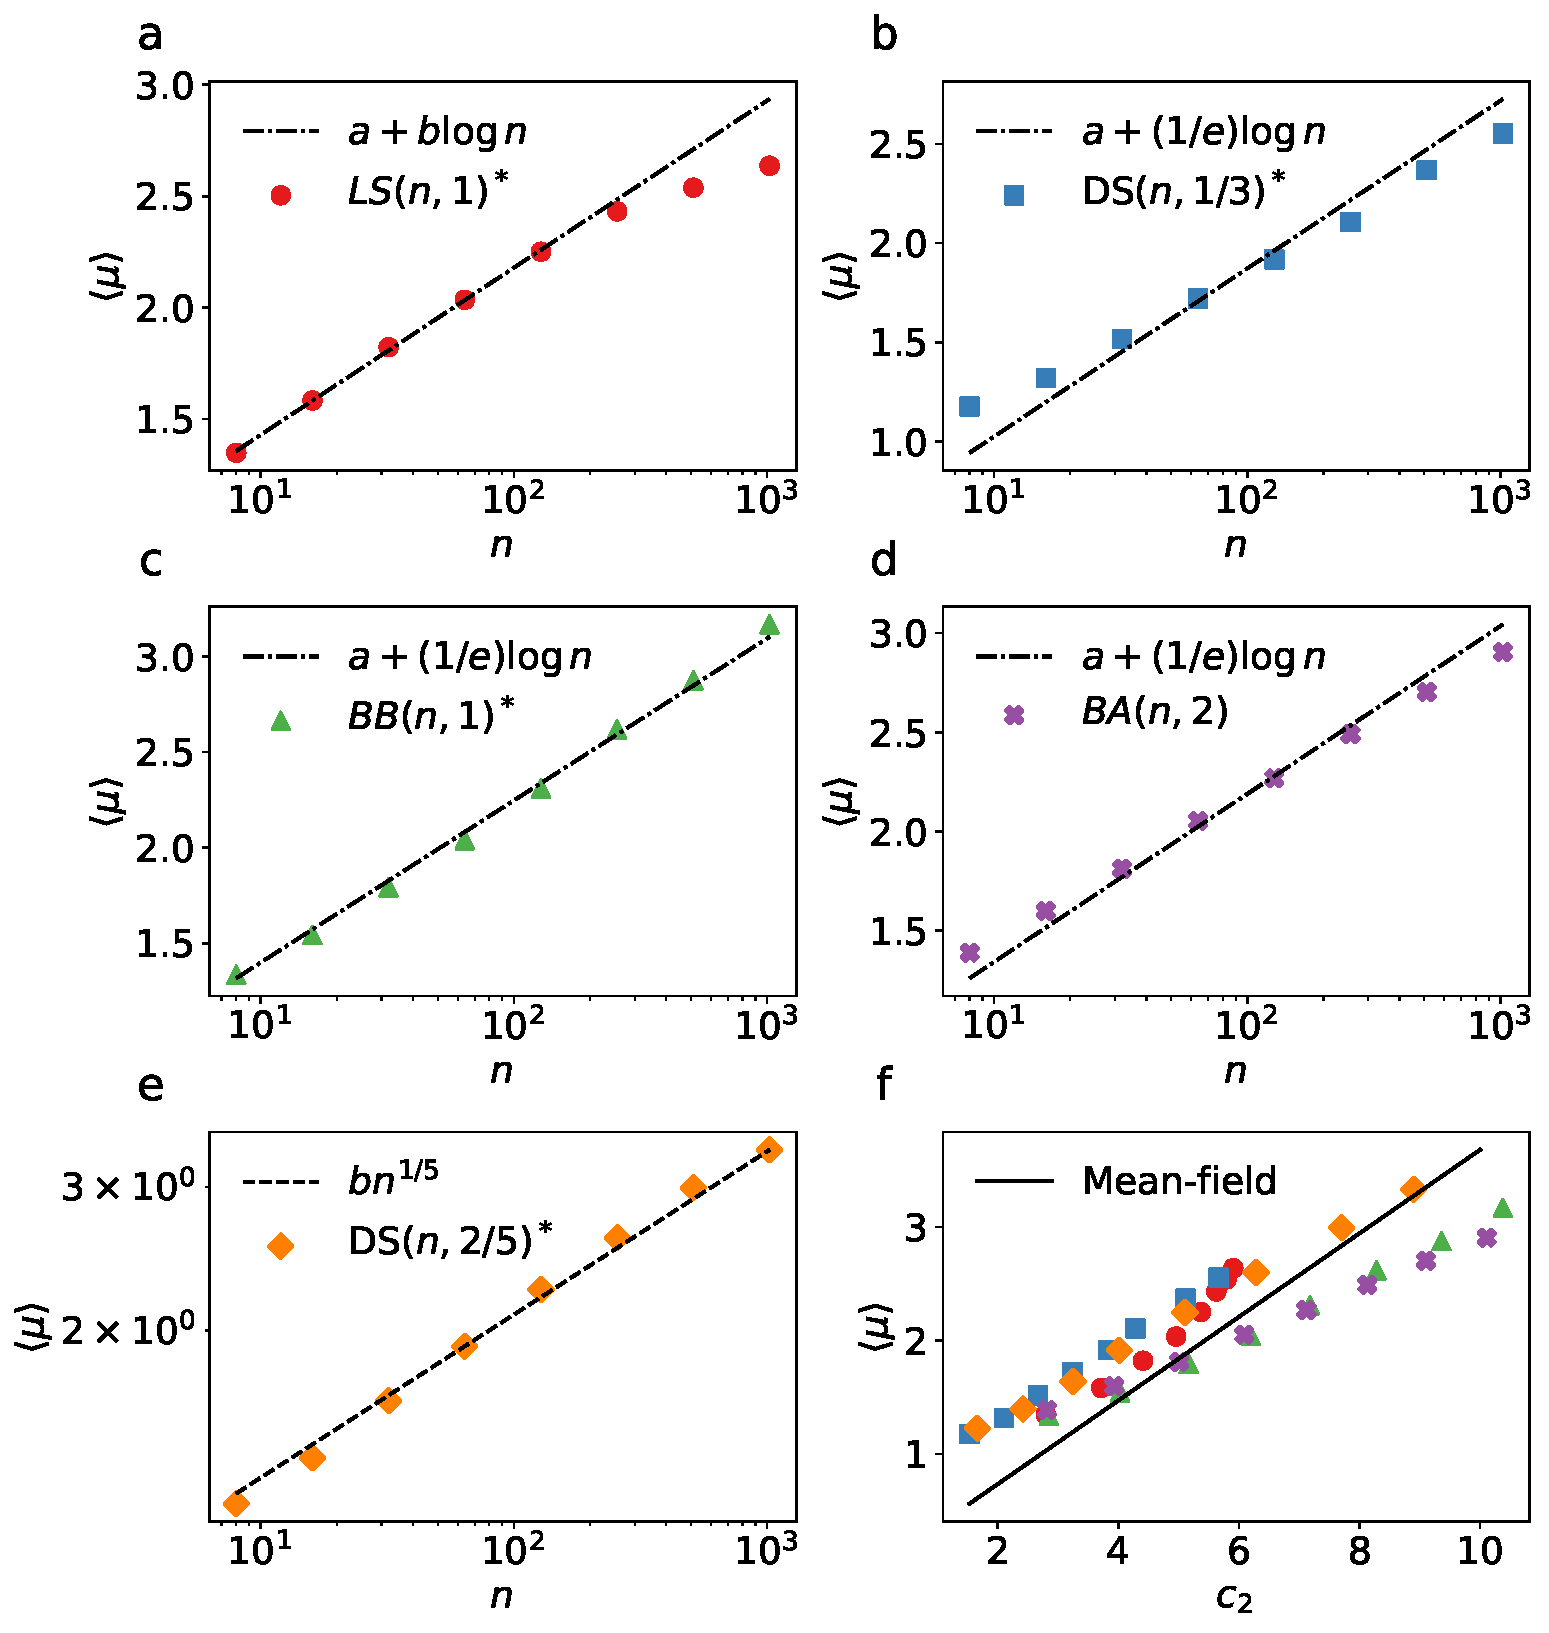
\includegraphics[width=3.4in]{fig1.pdf}
\caption{Scaling between the average shortest path multiplicity $\langle \mu\rangle$ and the network size $n$ for randomized networks. The networks were generated using the local rule indicated in the legend and then randomized by the degree preserving link rewiring. The lines highlight the logarithmic scaling.}
\label{fig_randomized}
\end{figure}

\section{Non-structured networks}
\label{random}

Dong {\em et al} \cite{dong2025multi} have estimated the network size scaling of the average shortest path multiplicity  for the Erd\"os-R\'enyi random graph model $ER(n, p)$, denoted by $\langle \mu\rangle_{ER}$. In the dense regime, $p$ near and above 0.1, $\langle \mu\rangle_{ER}$ scales linearly with $n$. However, real networks are sparse, corresponding to $p\sim1/n$.

To investigate sparse random networks, we can use as starting point the local rule models and then we apply the degree preserving link rewiring method. Figure \ref{fig_randomized} shows the average shortest path multiplicity $\langle \mu\rangle$ as a function of the network size $n$, the number of nodes. For all the sparse random networks tested there is a logarithmic growth
%
\begin{equation}
\langle \mu\rangle_{S,0} = a + b\log n,
\label{mu_rnd} 
\end{equation}
%
as it is emphasized by the fitted line in the semi-log plot. That is indeed slower than the linear dependency for the Erd\"os-R\'enyi graphs in the dense regime. The subscript {S0} stands for sparse network (S) and non-structured network (0). 

\begin{figure}
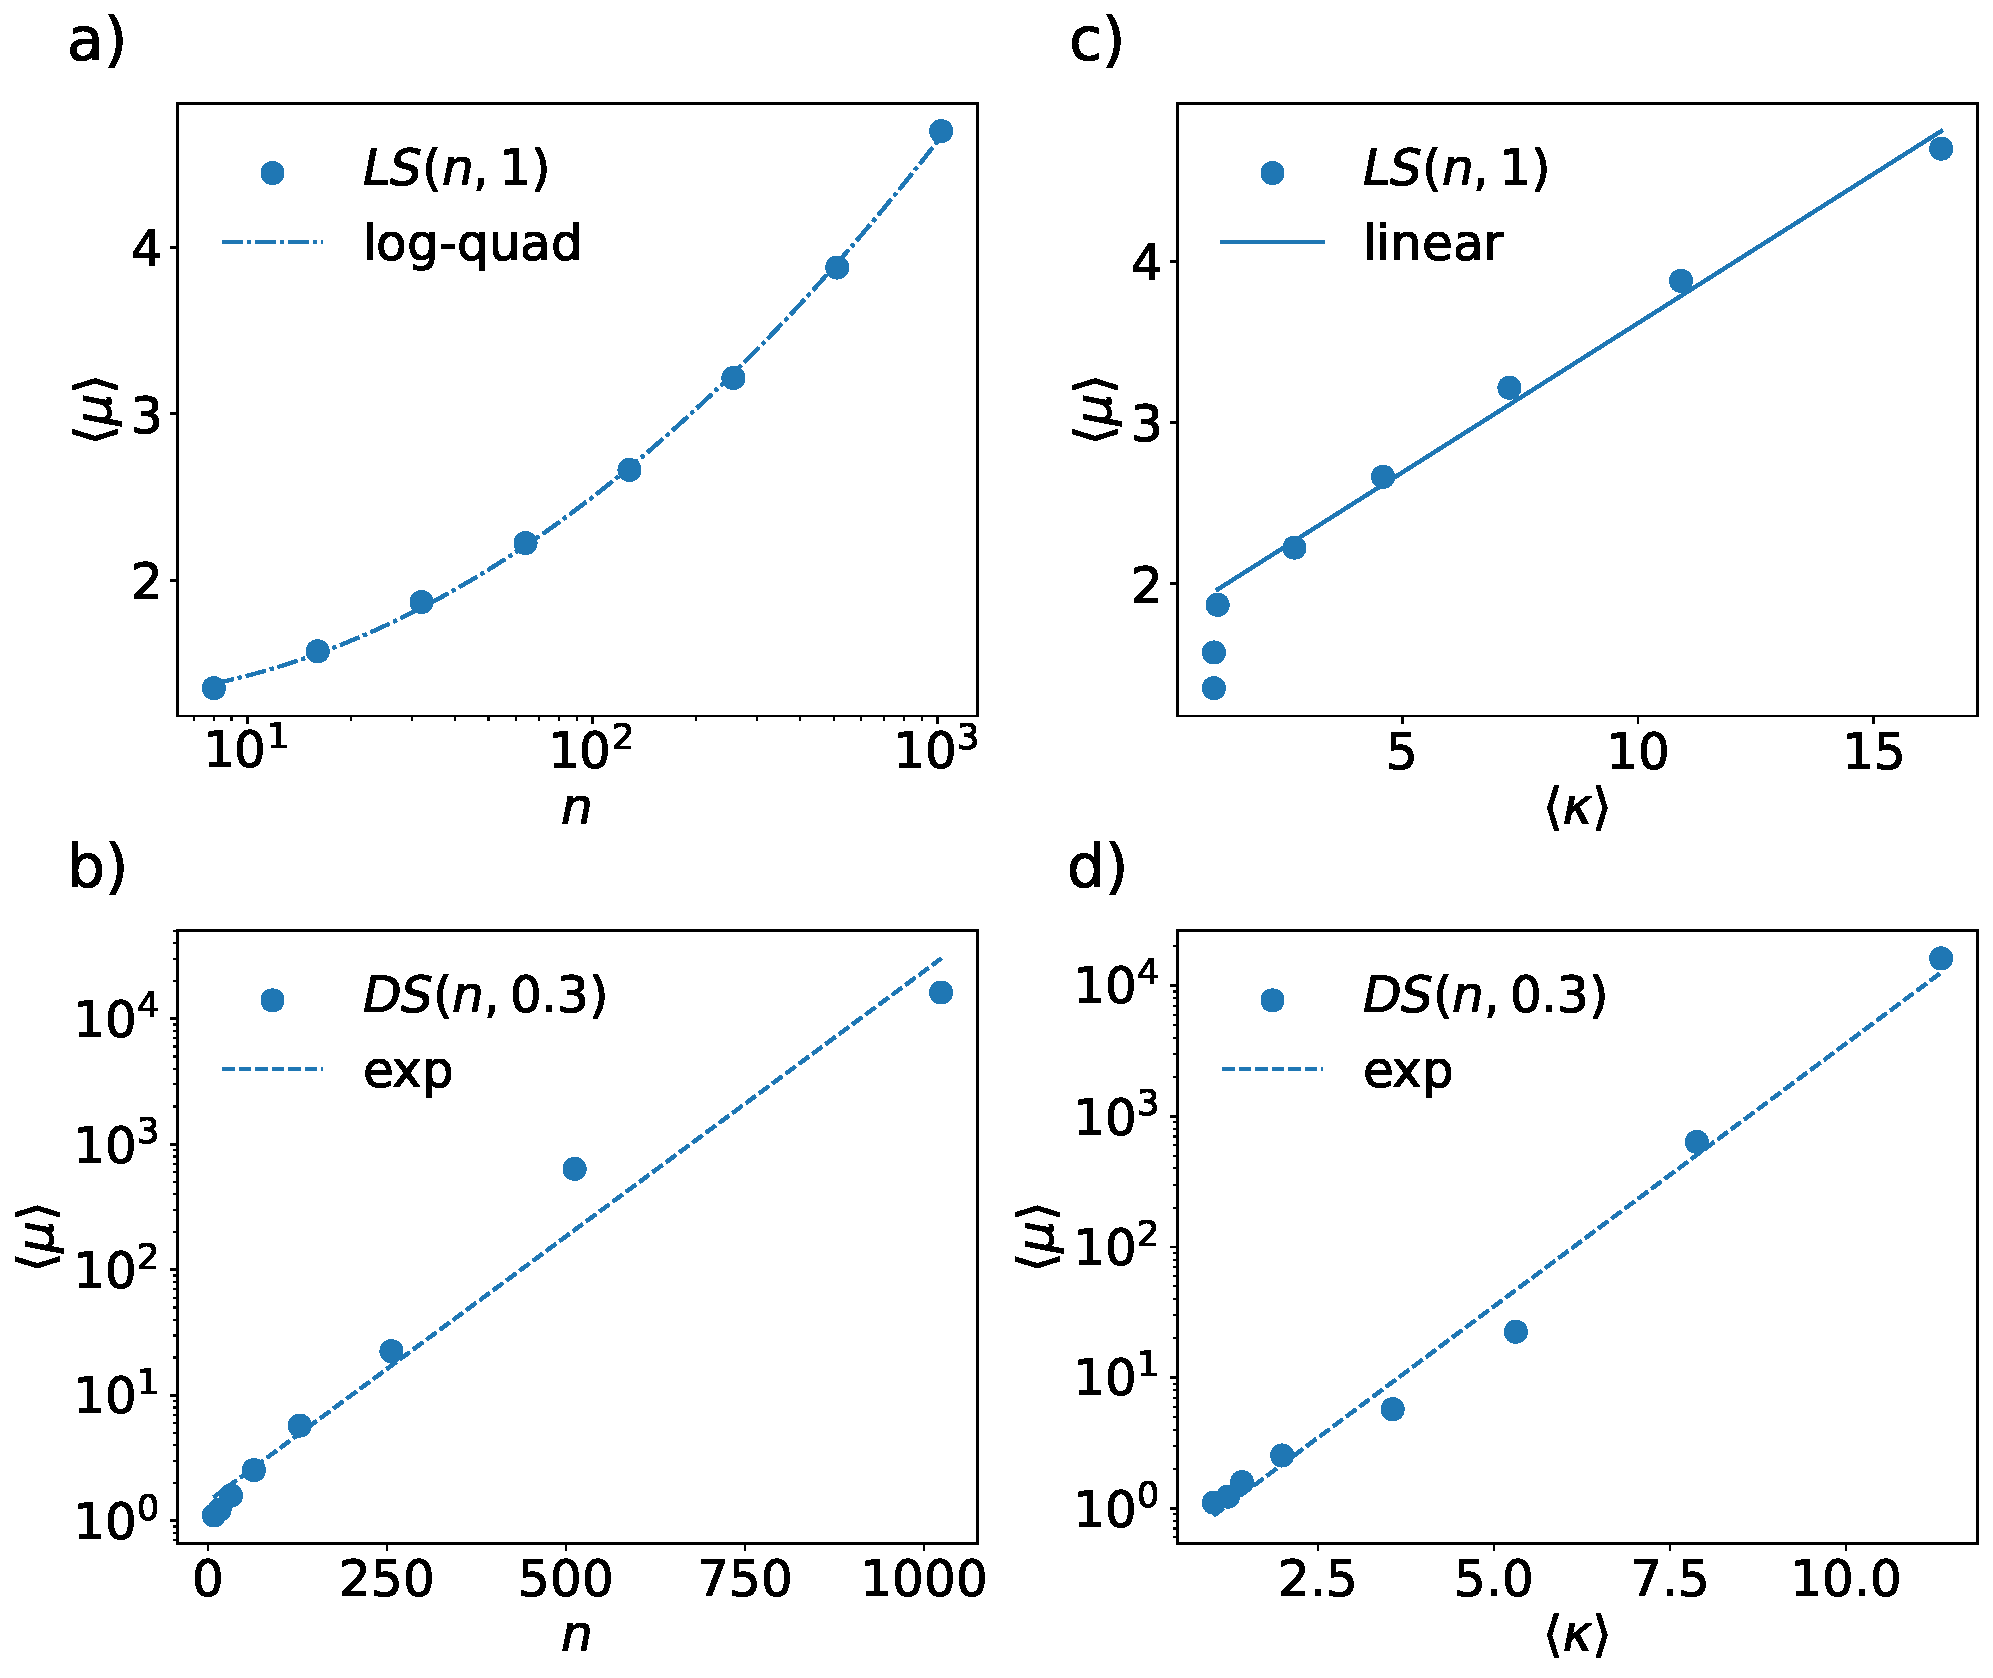
\includegraphics[width=3.4in]{fig2.pdf}
\caption{Scaling between the average shortest path multiplicity $\langle \mu\rangle$ and the network size $n$ for networks generated by the local-search and duplication-split local rules. The lines highlight the scaling specified in the legend. Note that it takes a critical network size $r_\kappa$ to detect network communities. Therefore, the scaling between $\langle\mu\rangle$ vs $\langle\kappa\rangle$ manifests for the largest network sizes simulated.}
\label{fig_local}
\end{figure}

\section{Networks with local structures}
\label{local}

Now we investigate the networks generated by the local rules, without rewiring. Although these local rules do not contain any pre-defined community structure, the resulting networks have communities as determined by standard methods of network communities detection  \cite{vazquez2025local}. In fact, beyond a certain network size $r_{\kappa}$, the Ramsey community number, the observation of network communities is almost certain. Now we proceed to uncover the scaling of the average shortest path multiplicity with the network size and with the number of inferred communities.

In all models investigated $\langle\mu\rangle$ is an increasing function of $n$. Furthermore, for all the network models with local rules the  average number of inferred communities $\langle\kappa\rangle$ increases with increasing $n$ as well. As a consequence, we can investigate the implicit relation between $\langle\mu\rangle$ and $\langle\kappa\rangle$.

Figure \ref{fig_local}a and b reports the data for the $LS(n, d=1)$ model: node addition, link creation to a randomly chosen existing node, local search stopping at 1 step, and link addition to the reached node. For this model $\langle\mu\rangle$ increases faster than linear with increasing $\log n$. A fit to the log-quadratic law
%
\begin{equation}
\langle\mu\rangle_{S,I} = a + b \log n + c (\log n)^2,
\label{mu_s1} 
\end{equation}
%
is consistent with the data points for the range of network sizes tested (Fig. \ref{fig_local}a, line). In turn, $\langle\mu\rangle$ exhibits a linear scaling with $\langle\kappa\rangle$ (Fig. \ref{fig_local}b).

Figure \ref{fig_local}c and d reports the data for the $DS(n, q=0.3)$ model: node addition and either node duplication with probability $q$, or link split otherwise. For this model $\langle\mu\rangle$ increases exponentially with $n$
%
\begin{equation}
\langle\mu\rangle_{S,II} = a e^{ b n},
\label{mu_s2} 
\end{equation}
%
where $a>0$ and $b>0$ (Fig. \ref{fig_local}c). $\langle\mu\rangle$ also exhibits an exponential scaling with $\langle\kappa\rangle$ (Fig. \ref{fig_local}d).

\begin{figure}
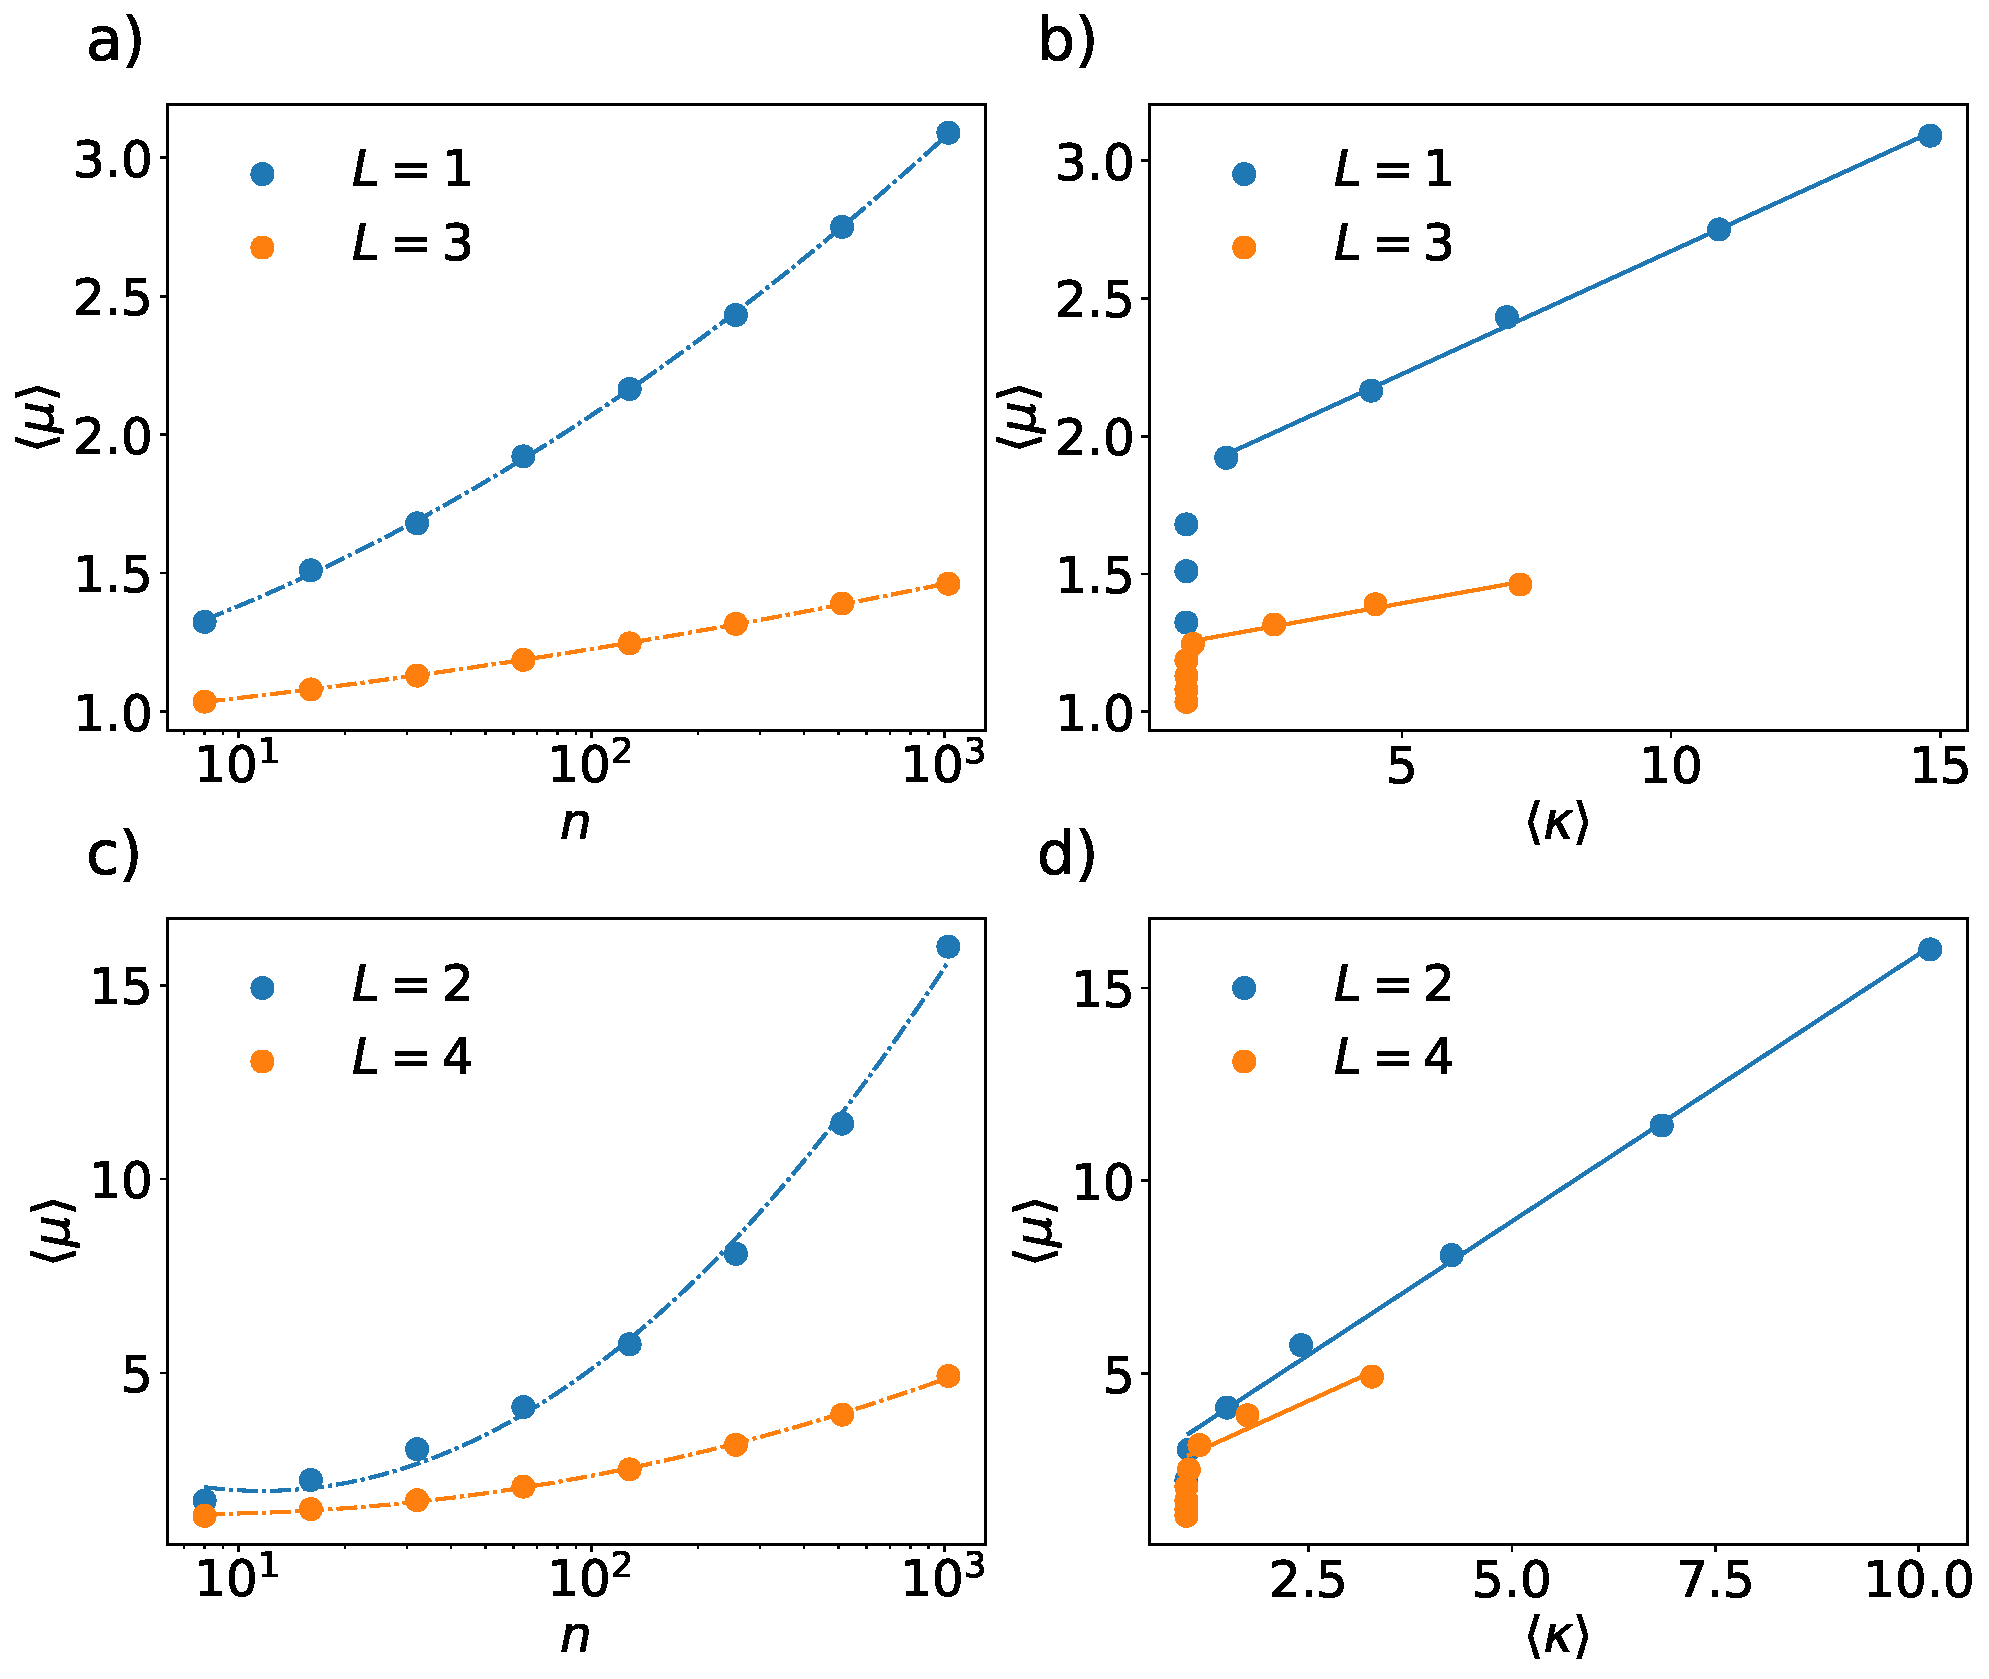
\includegraphics[width=3.4in]{fig3.pdf}
\caption{Scaling between the average shortest path multiplicity $\langle \mu\rangle$ and the network size $n$ for networks generated by the $BB(n, L)$ model. The lines highlight the scaling specified in the legend. Note that it takes a critical network size $r_\kappa$ to detect network communities. Therefore, the scaling between $\langle\mu\rangle$ vs $\langle\kappa\rangle$ manifests for the largest network sizes simulated.}
\label{fig_bubble}
\end{figure}

The differences between the local-search and duplication-split models could be related to the typical cycle length induced by the local rule. The triadic closure rule of $LS(n, 1)$ creates cycles of length 3. There is only one shortest path between the nodes in a 3-nodes cycle. In contrast, the duplication rule create cycles of length 4. Each node in a 4-cycle has two shortest paths to the opposite node two steps away. The duplication rule boosts the shortest path multiplicity. Note that this reasoning does not take into account the creation of multiple paths between existing nodes and passing through the new node, or between the new node and other existing nodes in the network. Such additional contribution is responsible for the type I scaling for the $LS(n, 1)$ networks.

The bubble model $BB(n, L)$ is a great tool to investigate the cycle length dependency. At each network update, a chain of $L$ nodes is connected to the ends of a randomly chosen link, thus forming a cycle of length $L+2$. For $L=2k-1$ with $k=1, 2,\ldots$ the bubble model generates cycles of odd length. Otherwise, for $L=2k$ with $k=1, 2,\ldots$  the cycles have even length. Based on the numerical simulations, $\langle\kappa\rangle$ reaches higher values for even $L$ than for odd $L$ (Fig. \ref{fig_bubble}). However, regardless of the $L$ parity, the scaling is log-quadratic, Eq. (\ref{mu_s1}) .

The exponential law Eq. (\ref{mu_s2}) should be rooted in some other aspect of the duplication rule. If the duplicated node has degree $k$ then it creates $k(k-1)/2$ squares. In turn there is preferential attachment. The link addition rate is $\pi_k = qk/n$. Using the rate equations for the nodes degree dynamics one obtains a power law degree distribution $p_k\sim k^{-\gamma}$ with $\gamma=1+1/q$. The average excess degree $\langle k(k-1)\rangle/2$ diverges with increasing $n$ for $q\geq 1/2$. Yet, we observe the exponential dependency in Eq. (\ref{mu_s2}) for $q=0.3$, where  $\langle k(k-1)\rangle/2$ is finite. The reason for the exponential scaling remains to be uncovered.

\begin{figure}
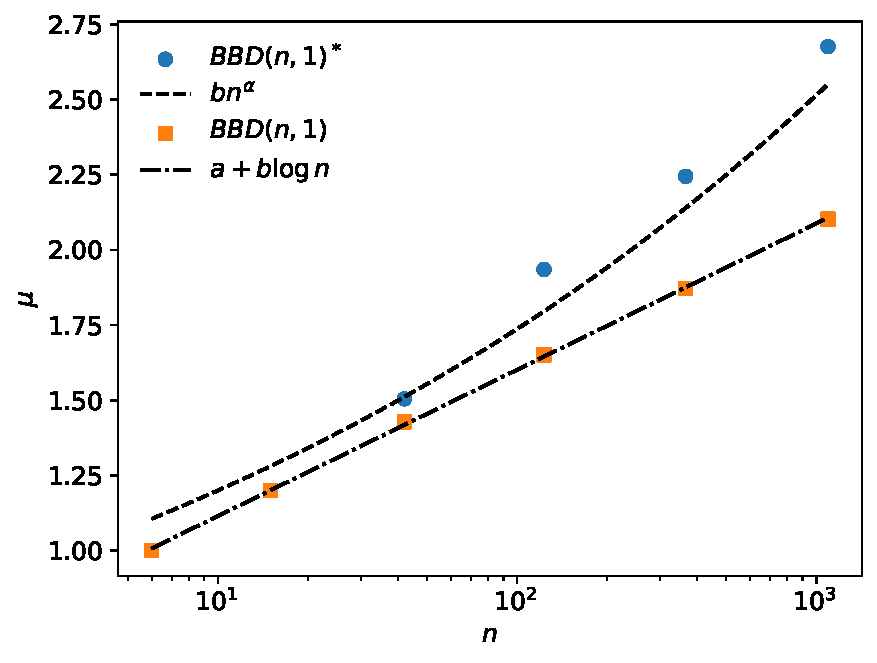
\includegraphics[width=3.4in]{fig4.pdf}
\caption{Scaling between the average shortest path multiplicity $\langle \mu\rangle$ and the network size $n$ for networks generated by the deterministic bubble model. The line highlights the log-linear scaling.}
\label{fig_deterministic}
\end{figure}

\section{Deterministic model}

Dorogovtsev, Goltsev and Mendes introduced a deterministic model for network growth with a recursive rule similar to the bubble model with $L=1$ \cite{dorogovtsev2002fractal}. The model is started at step $t=0$ with 3 connected nodes making a triangle. At each new step, new nodes are connected to both ends of every link in the current network. Given this deterministic recursion many properties can written down as a function of the step $t$ \cite{dorogovtsev2002fractal}.  I have attempted to derive a close expression between $\langle\mu\rangle$ and $n$, but I have failed. Surprisingly, the numerical results are better fitted by a log-linear relation, as observe for randomized networks (Fig. \ref{fig_deterministic}). This would suggest that the stochasticity of the local models plays some role in the observed log-quadratic scaling (Eq. \ref{mu_s1}). 

\section{Conclusions}
\label{conclusions}

In sparse networks without local structure, the average shortest path multiplicity $\langle\mu\rangle$ scales logarithmically with the network size $n$: $\langle\mu\rangle_{S,0} = a + b\log n$.

In sparse networks generated by local evolution rules,  we observe two types of scaling of the average shortest path multiplicity $\langle\mu\rangle$ vs $n$. For most models there is a log-quadratic scaling $\langle\mu\rangle_{S,I}= a + b\log n + c(\log n)^2$. In contrast, for the duplication-split model, a faster exponential growth $\langle\mu\rangle_{S,II} = a e^{bn}$ manifests.

Since the local evolution rules induce (i) the formation of network communities and (ii) the average number of communities $\langle\kappa\rangle$ increases with increasing the network size, then we can investigate the scaling between $\langle\mu\rangle$ and $\langle\kappa\rangle$. It is linear for all models tested, except for the duplication-split model where an exponential dependency was observed.

We could say local evolution rules and network communities are two sides of the same coin. With that view in mind, the statements that local evolution rules increase shortest path multiplicity and that network communities increase shortest path multiplicity  are equivalent. However, we should bear in mind that the local network evolution rules model the natural evolution of the systems they represent. In that regard, the local evolution rules are the driving mechanism and everything else follows.


\bibliographystyle{apsrev4-1}

%\bibliography{network.bib}

\documentclass[reprint,aps,pre,amsmath,amssymb,superscriptaddress,showpacs]{revtex4-1}
\usepackage{graphicx}
\usepackage{hyperref}
\usepackage{color}

\newtheorem{definition}{Definition}

\begin{document}

\title{Local network evolution rules drive shortest path multiplicity}

\author{Alexei Vazquez}
\email{alexei@nodeslinks.com}
\affiliation{Nodes \& Links Ltd, Salisbury House, Station Road, Cambridge, CB1 2LA, UK}

\begin{abstract}
The shortest path multiplicity is an important metric of complex networks. The shortest path multiplicity of real networks is high and it correlates with their community structure. Since local network evolution induces network communities, it is possible that a high shortest path multiplicity is the natural expectation of local evolution rules. Here I demonstrate, by means of numerical simulations, that this is indeed the case.
\end{abstract}

\maketitle

\section{Introduction}

The fundamental question of network science is to determine the minimum set of properties and models to explain what we observe in real networks. New discoveries should be subject to the scrutiny of existing concepts. That is the case of the  recent observation by Deng {\em et al} \cite{deng2026multipath}, a correlation between the number of communities and the density of multiple shortest paths in real networks. This correlation could be the consequence of an upstream factor that causes both features. And it turns out that there is an obvious candidate: local evolution rules.

Local network evolution rules are node/link addition mechanisms of network growth \cite{vazquez03local}. Local rules are inspired by the natural evolution of real networks. Web pages are created by copying other pages \cite{kleinberg99}. We cite references that we found reading another publication \cite{vazquez01rs}. Friends of friends become friends \cite{growing_social_networks_jin01}.  Proteins increase their connectivity when their interacting partners are duplicated \cite{vazquez03dup, pastor-satorras03}. Local evolution rules lead to the emergence of network communities: beyond a certain network size we can warrant that the network will exhibit communities \cite{vazquez2025local}. These communities are not written in the network evolution rules. Yet they are imputed by the state of the art methods to detect network communities.

Local evolution rules induce the formation of short cycles and cycles tend to increase the shortest path multiplicity. Therefore, I raise the hypothesis that the high shortest path multiplicity of real networks is rooted on their local growth dynamics. Furthermore, since those local rules induce the formation of networks communities, that would explain the association between shortest path multiplicity and network communities as well.

In this work I investigate this hypothesis by means of numerical simulations. In the Sec. \ref{methods} I introduce different models of growing networks with local rules and the methods used to quantify their properties. In Sec. \ref{random} I characterize random networks without local structures to set the baseline expectation. In Sec. \ref{local} I characterize the networks generated by local rules. The concluding remarks are reported in Sec. \ref{conclusions}.

\section{Methods}
\label{methods}

The computer code related to these methods is available at \href{https://github.com/av2atgh/ramsey_netcom}{github.com/av2atgh/ramsey\_netcom}.

\subsection{Local models}

Local search $LS(n, d)$. {\em Initial condition}. The network is started with two connected nodes. Evolution rule: A new node is added and a $d$-step random walk is performed from a randomly selected node in the current network. The new node is connected to all
visited nodes. This model has preferential attachment because the probability that a node is visited, beyond the entry node, is proportional to the current nodes degrees. Consequently it generate networks with a power law degree distribution. The $LS(n, d)$ networks have a
high clustering coefficient. At least 1 triangle, between the entry point and next neighbor visited, is formed at every node addition. For $d=1$ this model is equivalent to the triadic closure model \cite{growing_social_networks_jin01, communities_bianconi_2014}.

Duplication split $DS(n, q)$. {\em Initial condition}: The network is started with two connected nodes. {\em Evolution rule}: A new node $i$ is added to the network and a node in the current network is selected at random, node $j$. With probability $q$, $i$ becomes a duplicate of $j$ with links from $i$ to all neighbors of $j$. Otherwise, a link between $j$ and a randomly selected neighbor of $j$, node $k$, is split. The edge $(j, k)$ is removed and new edges $(i, j)$ and $(i, k)$ are created. This model has preferential attachment because, for the duplication rule, the probability that a node neighbor is duplicated is proportional to the node degree. The duplication rule does not make triangles and the split rule breaks triangles if they would exist. The main motif of this model is the formation of squares (cycles of length 4) between any two neighbors of the reference node $j$ and its duplicate $i$.

Bubble model $BB(n, L)$. {\em Initial condition}: The network is started with two connected nodes. {\em Evolution rule}: A chain of $L$ new nodes is added to the network. The two nodes at the chain ends are attached to the ends of an existing link, creating a cycle of length $L+2$. $BB(n, 1)$ is equivalent to an earlier Dorogovtsev-Mendes model where new nodes are connected to both ends of a randomly chosen link by two undirected links \cite{dorogotsev2001link}. The model has preferential attachment because the probability that a node is at the end of the selected link is proportional to its degree. The main network motif are the cycles of length $L+2$ created by the evolution rule.

All these models have a finite Ramsey community number $r_\kappa$, the minimum graph size that guarantees the emergence of network communities with almost certainty \cite{vazquez2025local}.

\subsection{Network communities}

The network communities are inferred using the stochastic block model implemented in graph-tool (\verb|graph_tool.inference.minimize_blockmodel_dl|, with default parameters) \cite{peixoto_graph-tool_2014}. This stochastic block model finds the community structure with the minimum description length \cite{peixoto2024networkreconstructionminimumdescription}. In that sense, it gives as output the optimal number of communities $\kappa$ and the partition of the nodes into communities. The average of $\kappa$ is calculated from 100 realizations of network creation plus network community inference.

An important parameter is the correction for the network degree sequence, \verb| deg_corr: bool (optional, default: True)|. Some of the networks investigated have power law degree distributions, and therefore I use the degree-corrected version of the stochastic block model (default option). Similar results are obtained using the Infomap method implemented in the package with the same name \cite{mapequation2025software}, as previously shown \cite{vazquez2025local}.

\subsection{Network rewiring}

For network rewiring, I use the standard configuration model implemented with \verb|graph_tool.generation.random_rewire| with default parameters. The configuration algorithm rewires the network links preserving the degree distribution \cite{configuration_method_park_2004}.

\subsection{Shortest path multiplicity}

To determine the path multiplicity $\mu_{ij}(G)$ between a pair of nodes $(i, j)$ in graph $G$, I use the graph-tool method \verb|graph_tool.count_shortest_paths(G, i, j)| with default parameters.

Given a graph generator $f_G$, I calculate the average shortest path multiplicity $\langle \mu\rangle$ as the average over every pair of nodes and over 100 realizations of $G$.

\begin{figure}
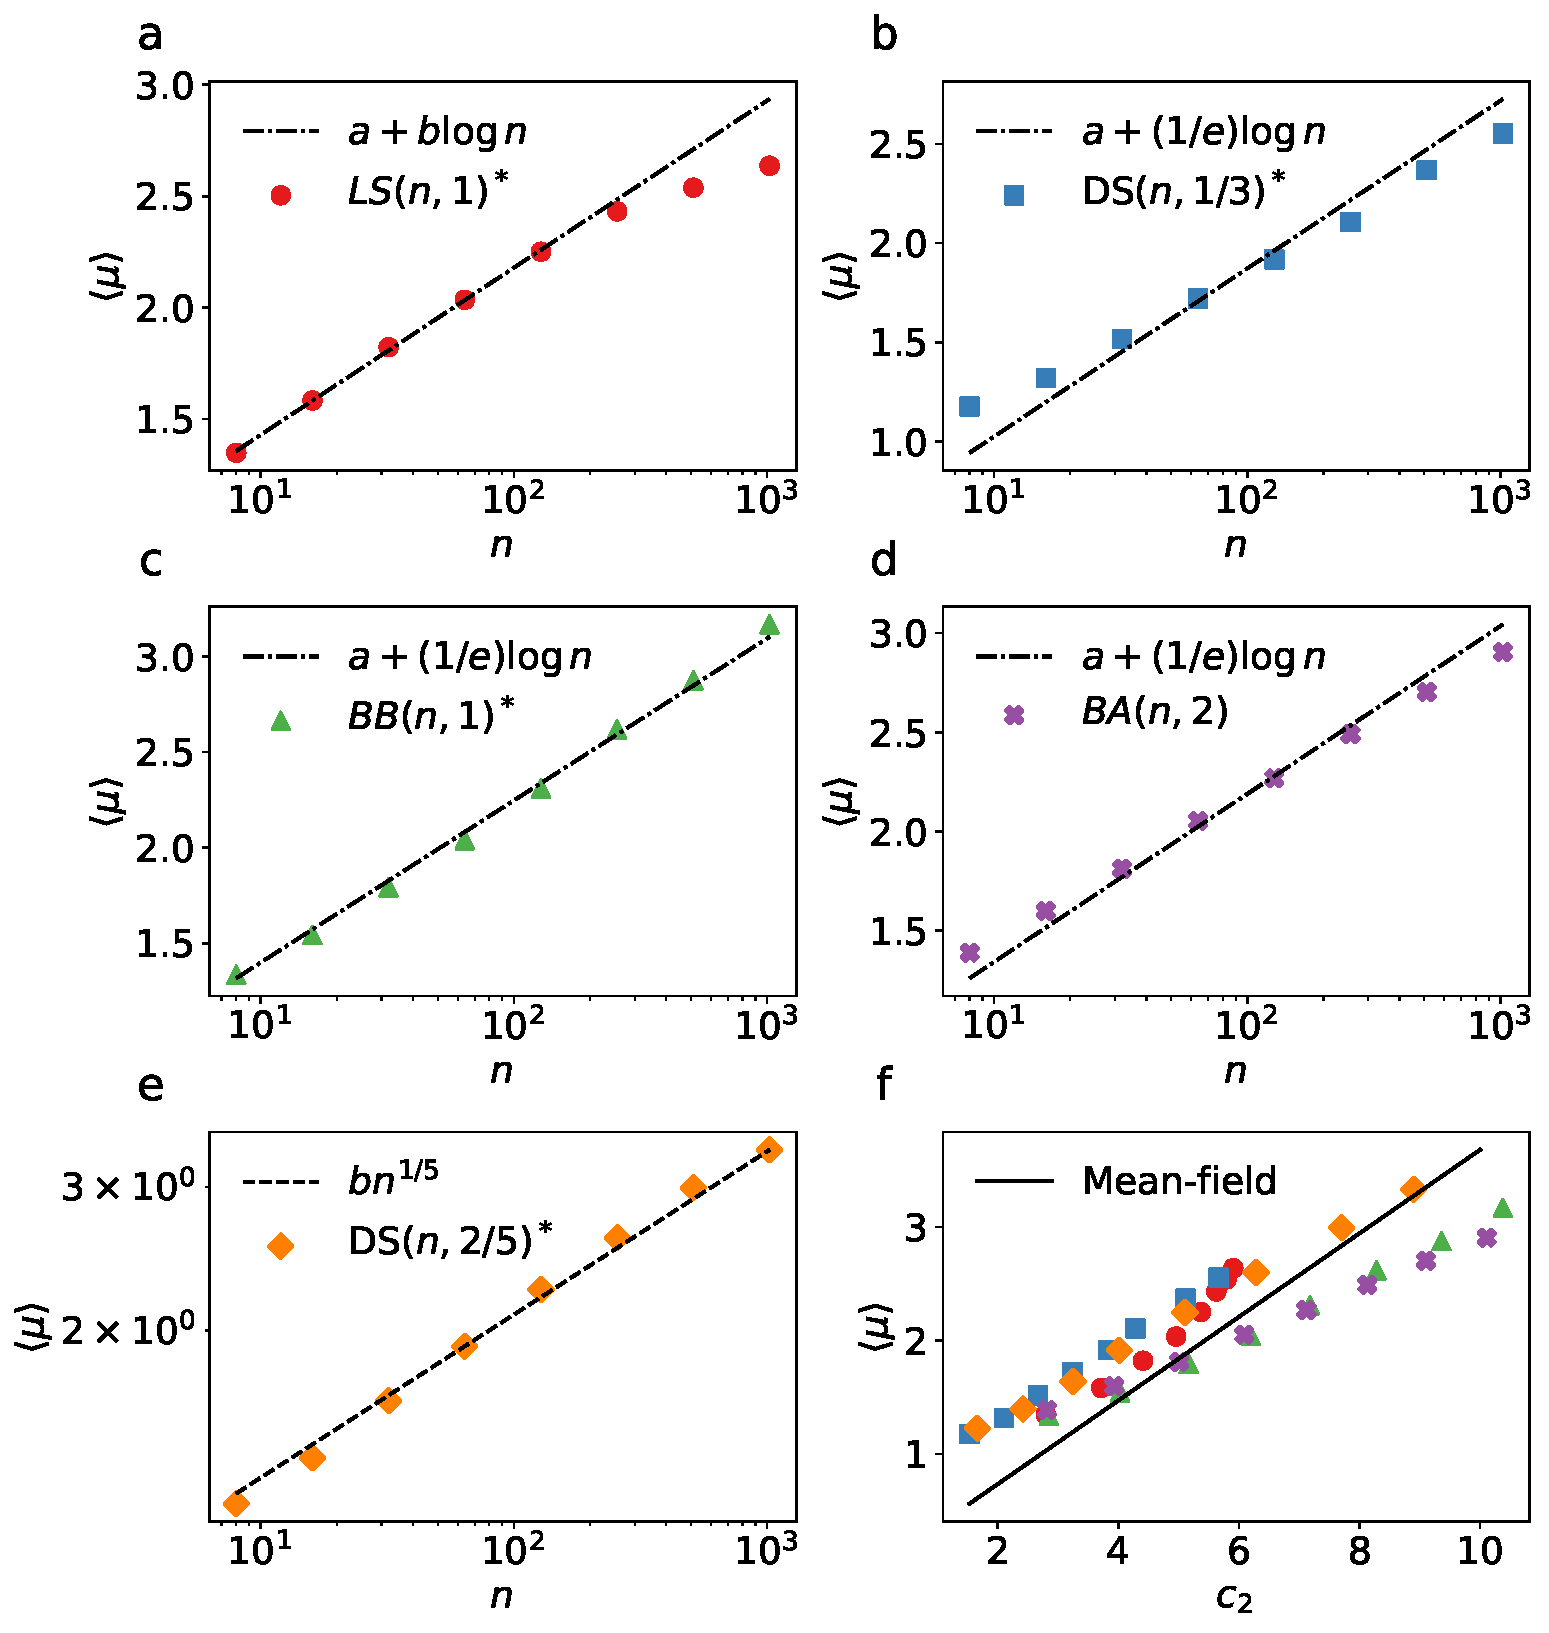
\includegraphics[width=3.4in]{fig1.pdf}
\caption{Scaling between the average shortest path multiplicity $\langle \mu\rangle$ and the network size $n$ for randomized networks. The networks were generated using the local rule indicated in the legend and then randomized by the degree preserving link rewiring. The lines highlight the logarithmic scaling.}
\label{fig_randomized}
\end{figure}

\section{Non-structured networks}
\label{random}

Dong {\em et al} \cite{dong2025multi} have estimated the network size scaling of the average shortest path multiplicity  for the Erd\"os-R\'enyi random graph model $ER(n, p)$, denoted by $\langle \mu\rangle_{ER}$. In the dense regime, $p$ near and above 0.1, $\langle \mu\rangle_{ER}$ scales linearly with $n$. However, real networks are sparse, corresponding to $p\sim1/n$.

To investigate sparse random networks, we can use as starting point the local rule models and then we apply the degree preserving link rewiring method. Figure \ref{fig_randomized} shows the average shortest path multiplicity $\langle \mu\rangle$ as a function of the network size $n$, the number of nodes. For all the sparse random networks tested there is a logarithmic growth
%
\begin{equation}
\langle \mu\rangle_{S,0} = a + b\log n,
\label{mu_rnd} 
\end{equation}
%
as it is emphasized by the fitted line in the semi-log plot. That is indeed slower than the linear dependency for the Erd\"os-R\'enyi graphs in the dense regime. The subscript {S0} stands for sparse network (S) and non-structured network (0). 

\begin{figure}
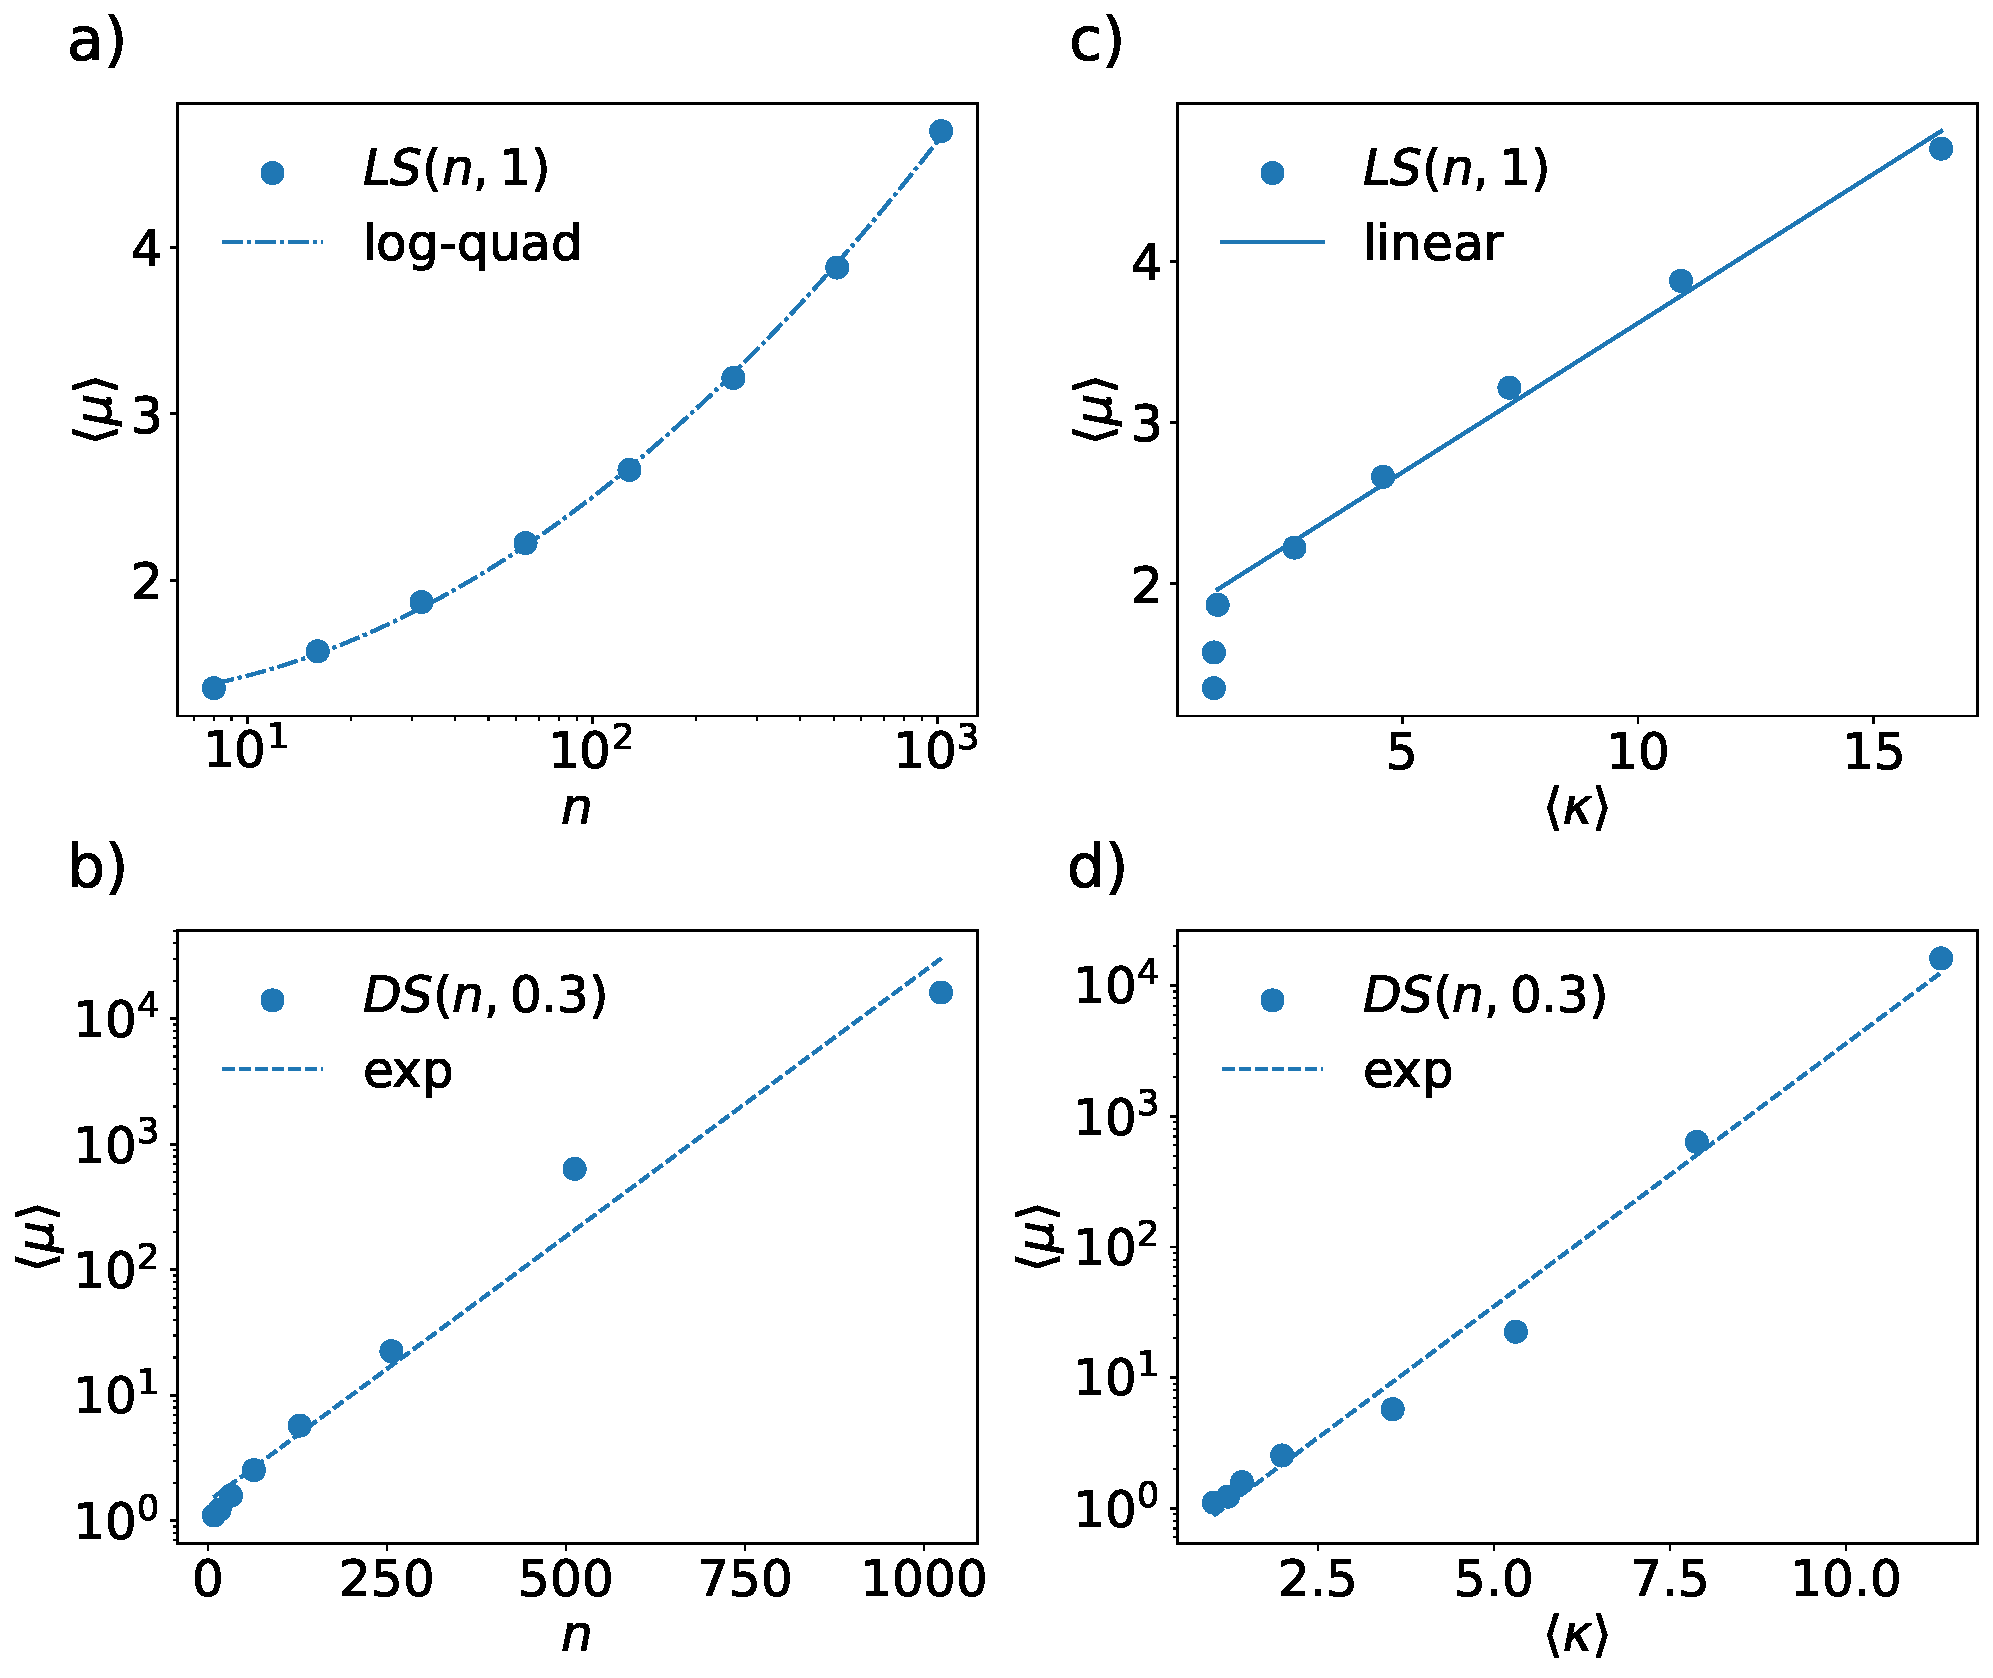
\includegraphics[width=3.4in]{fig2.pdf}
\caption{Scaling between the average shortest path multiplicity $\langle \mu\rangle$ and the network size $n$ for networks generated by the local-search and duplication-split local rules. The lines highlight the scaling specified in the legend. Note that it takes a critical network size $r_\kappa$ to detect network communities. Therefore, the scaling between $\langle\mu\rangle$ vs $\langle\kappa\rangle$ manifests for the largest network sizes simulated.}
\label{fig_local}
\end{figure}

\section{Networks with local structures}
\label{local}

Now we investigate the networks generated by the local rules, without rewiring. Although these local rules do not contain any pre-defined community structure, the resulting networks have communities as determined by standard methods of network communities detection  \cite{vazquez2025local}. In fact, beyond a certain network size $r_{\kappa}$, the Ramsey community number, the observation of network communities is almost certain. Now we proceed to uncover the scaling of the average shortest path multiplicity with the network size and with the number of inferred communities.

In all models investigated $\langle\mu\rangle$ is an increasing function of $n$. Furthermore, for all the network models with local rules the  average number of inferred communities $\langle\kappa\rangle$ increases with increasing $n$ as well. As a consequence, we can investigate the implicit relation between $\langle\mu\rangle$ and $\langle\kappa\rangle$.

Figure \ref{fig_local}a and b reports the data for the $LS(n, d=1)$ model: node addition, link creation to a randomly chosen existing node, local search stopping at 1 step, and link addition to the reached node. For this model $\langle\mu\rangle$ increases faster than linear with increasing $\log n$. A fit to the log-quadratic law
%
\begin{equation}
\langle\mu\rangle_{S,I} = a + b \log n + c (\log n)^2,
\label{mu_s1} 
\end{equation}
%
is consistent with the data points for the range of network sizes tested (Fig. \ref{fig_local}a, line). In turn, $\langle\mu\rangle$ exhibits a linear scaling with $\langle\kappa\rangle$ (Fig. \ref{fig_local}b).

Figure \ref{fig_local}c and d reports the data for the $DS(n, q=0.3)$ model: node addition and either node duplication with probability $q$, or link split otherwise. For this model $\langle\mu\rangle$ increases exponentially with $n$
%
\begin{equation}
\langle\mu\rangle_{S,II} = a e^{ b n},
\label{mu_s2} 
\end{equation}
%
where $a>0$ and $b>0$ (Fig. \ref{fig_local}c). $\langle\mu\rangle$ also exhibits an exponential scaling with $\langle\kappa\rangle$ (Fig. \ref{fig_local}d).

\begin{figure}
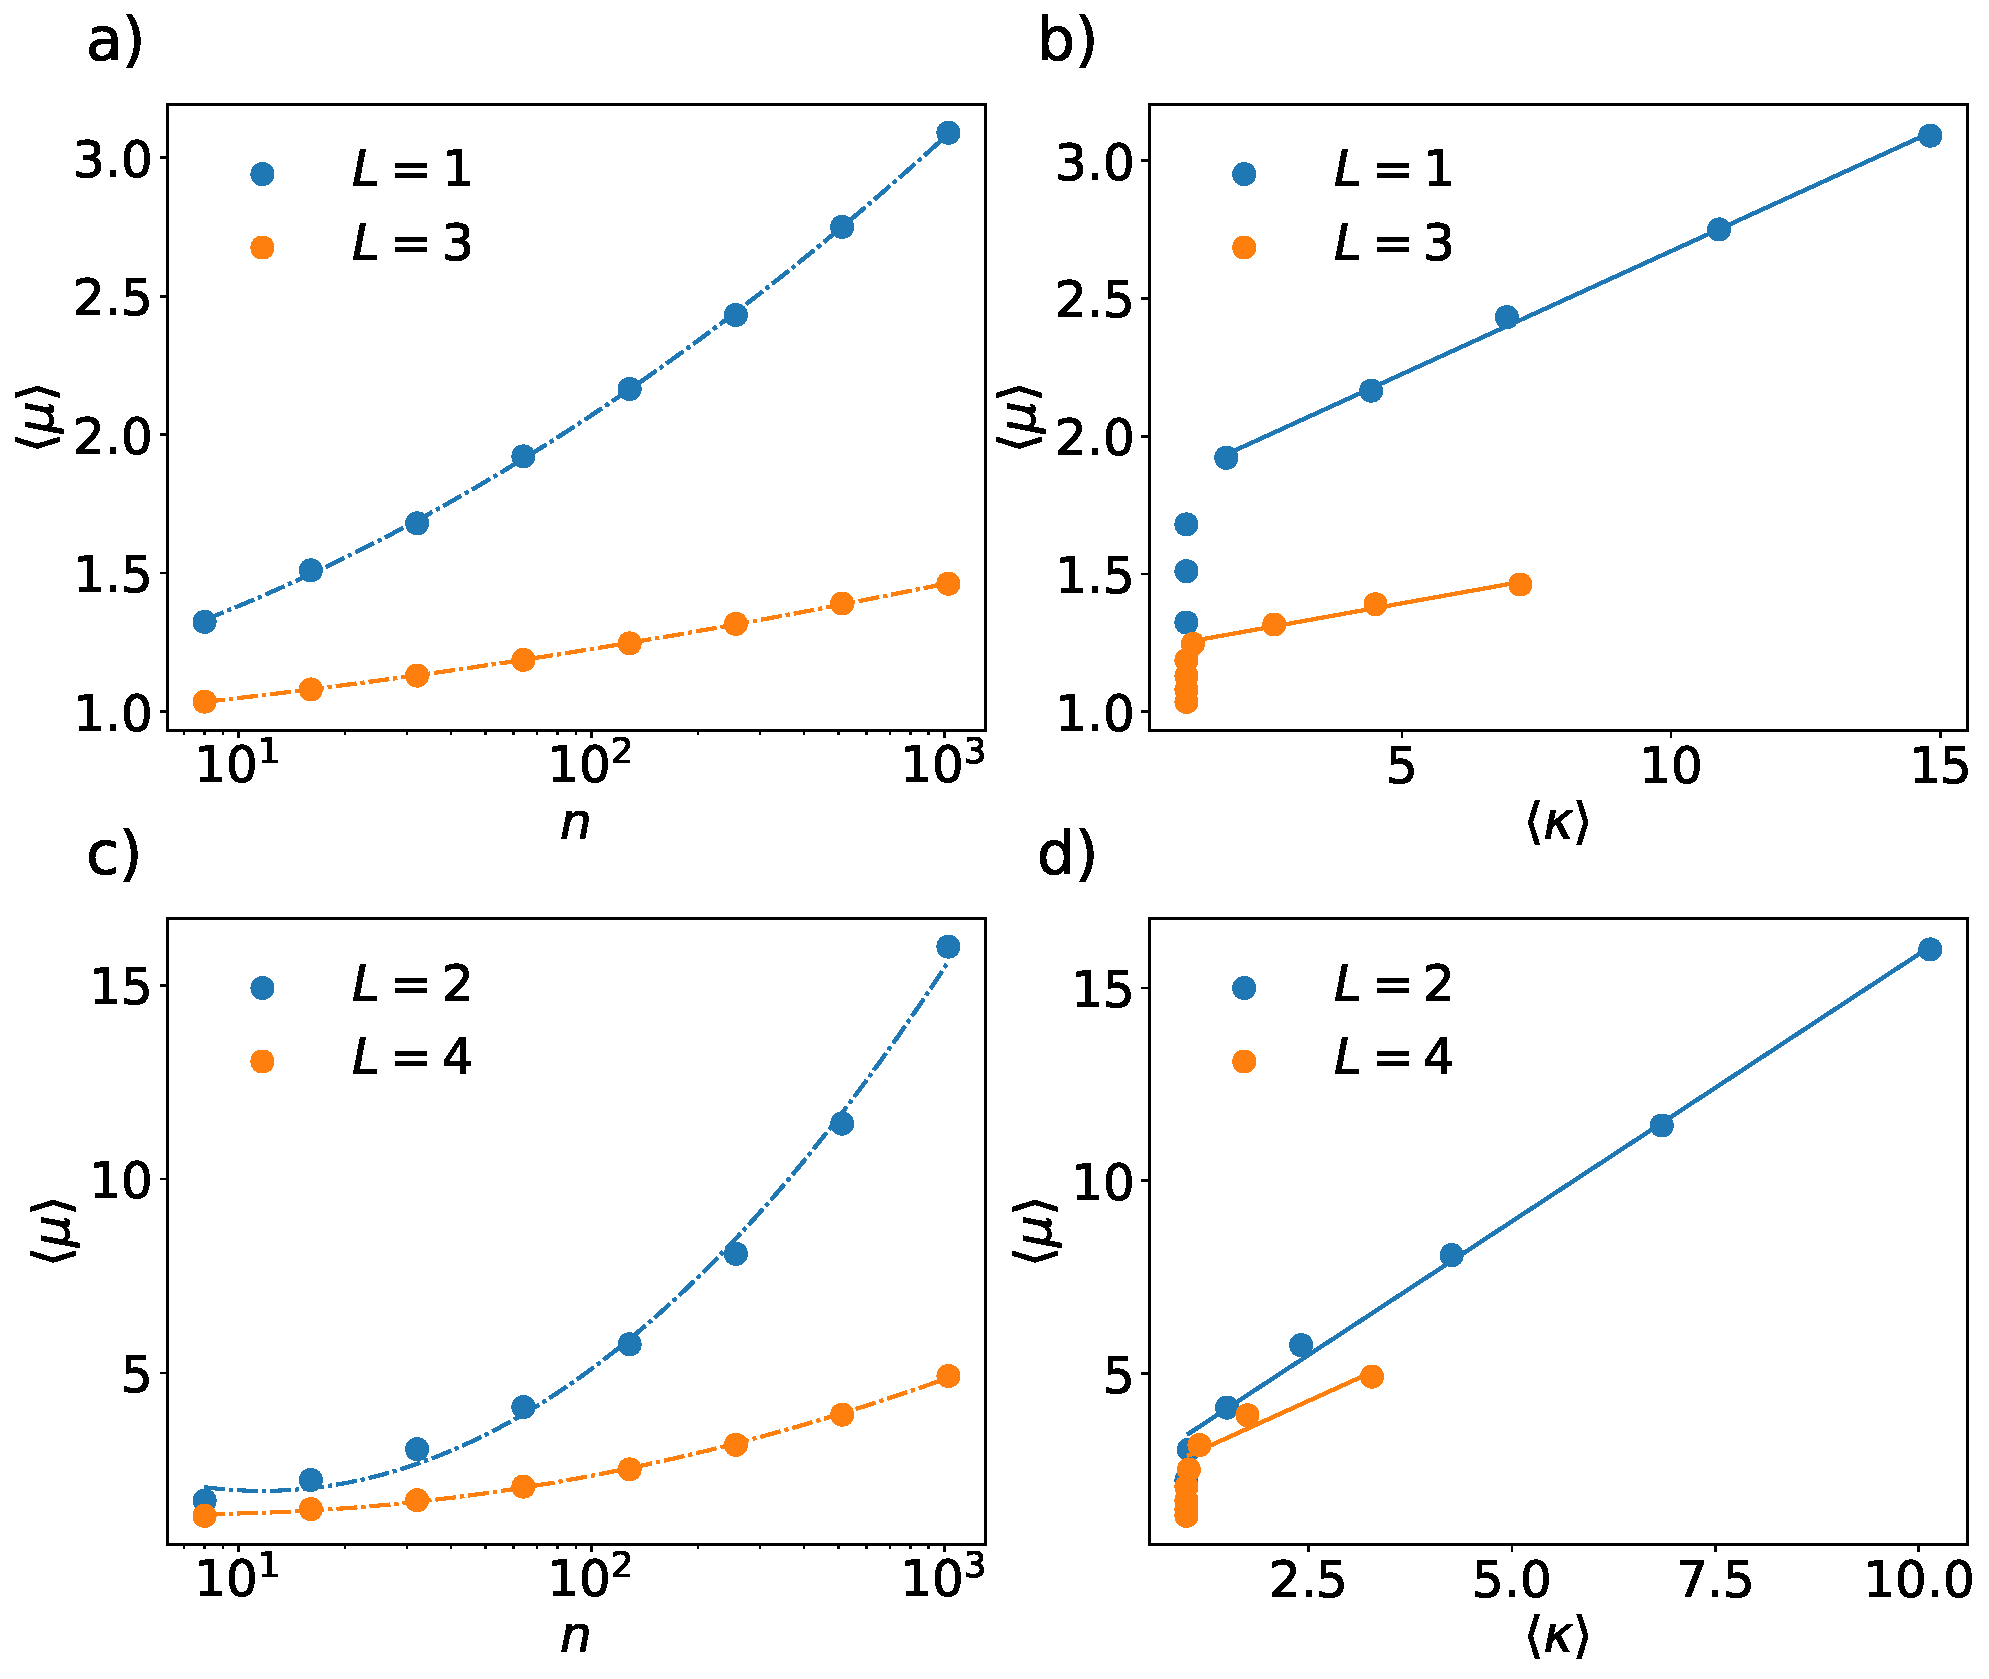
\includegraphics[width=3.4in]{fig3.pdf}
\caption{Scaling between the average shortest path multiplicity $\langle \mu\rangle$ and the network size $n$ for networks generated by the $BB(n, L)$ model. The lines highlight the scaling specified in the legend. Note that it takes a critical network size $r_\kappa$ to detect network communities. Therefore, the scaling between $\langle\mu\rangle$ vs $\langle\kappa\rangle$ manifests for the largest network sizes simulated.}
\label{fig_bubble}
\end{figure}

The differences between the local-search and duplication-split models could be related to the typical cycle length induced by the local rule. The triadic closure rule of $LS(n, 1)$ creates cycles of length 3. There is only one shortest path between the nodes in a 3-nodes cycle. In contrast, the duplication rule create cycles of length 4. Each node in a 4-cycle has two shortest paths to the opposite node two steps away. The duplication rule boosts the shortest path multiplicity. Note that this reasoning does not take into account the creation of multiple paths between existing nodes and passing through the new node, or between the new node and other existing nodes in the network. Such additional contribution is responsible for the type I scaling for the $LS(n, 1)$ networks.

The bubble model $BB(n, L)$ is a great tool to investigate the cycle length dependency. At each network update, a chain of $L$ nodes is connected to the ends of a randomly chosen link, thus forming a cycle of length $L+2$. For $L=2k-1$ with $k=1, 2,\ldots$ the bubble model generates cycles of odd length. Otherwise, for $L=2k$ with $k=1, 2,\ldots$  the cycles have even length. Based on the numerical simulations, $\langle\kappa\rangle$ reaches higher values for even $L$ than for odd $L$ (Fig. \ref{fig_bubble}). However, regardless of the $L$ parity, the scaling is log-quadratic, Eq. (\ref{mu_s1}) .

The exponential law Eq. (\ref{mu_s2}) should be rooted in some other aspect of the duplication rule. If the duplicated node has degree $k$ then it creates $k(k-1)/2$ squares. In turn there is preferential attachment. The link addition rate is $\pi_k = qk/n$. Using the rate equations for the nodes degree dynamics one obtains a power law degree distribution $p_k\sim k^{-\gamma}$ with $\gamma=1+1/q$. The average excess degree $\langle k(k-1)\rangle/2$ diverges with increasing $n$ for $q\geq 1/2$. Yet, we observe the exponential dependency in Eq. (\ref{mu_s2}) for $q=0.3$, where  $\langle k(k-1)\rangle/2$ is finite. The reason for the exponential scaling remains to be uncovered.

\begin{figure}
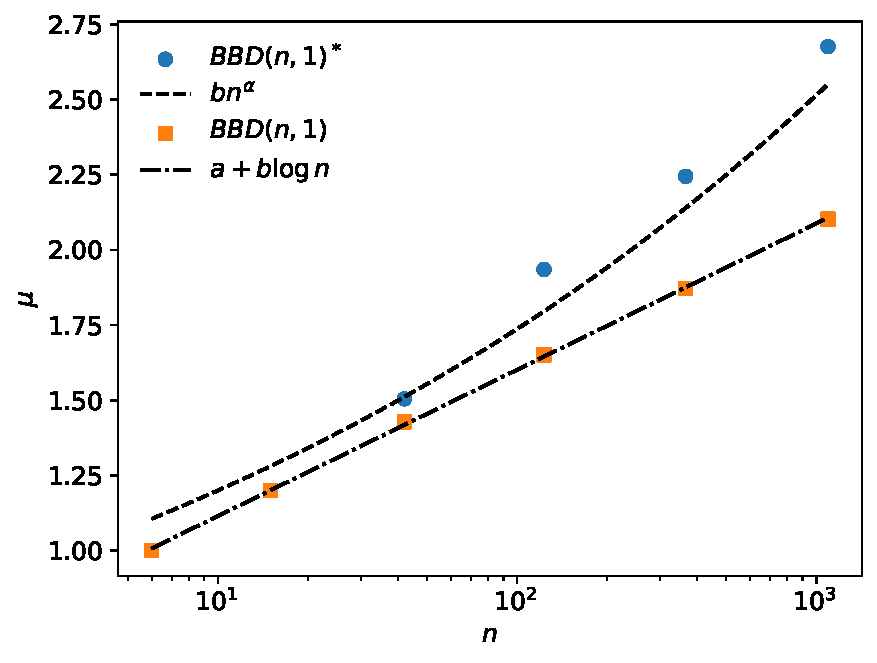
\includegraphics[width=3.4in]{fig4.pdf}
\caption{Scaling between the average shortest path multiplicity $\langle \mu\rangle$ and the network size $n$ for networks generated by the deterministic bubble model. The line highlights the log-linear scaling.}
\label{fig_deterministic}
\end{figure}

\section{Deterministic model}

Dorogovtsev, Goltsev and Mendes introduced a deterministic model for network growth with a recursive rule similar to the bubble model with $L=1$ \cite{dorogovtsev2002fractal}. The model is started at step $t=0$ with 3 connected nodes making a triangle. At each new step, new nodes are connected to both ends of every link in the current network. Given this deterministic recursion many properties can written down as a function of the step $t$ \cite{dorogovtsev2002fractal}.  I have attempted to derive a close expression between $\langle\mu\rangle$ and $n$, but I have failed. Surprisingly, the numerical results are better fitted by a log-linear relation, as observe for randomized networks (Fig. \ref{fig_deterministic}). This would suggest that the stochasticity of the local models plays some role in the observed log-quadratic scaling (Eq. \ref{mu_s1}). 

\section{Conclusions}
\label{conclusions}

In sparse networks without local structure, the average shortest path multiplicity $\langle\mu\rangle$ scales logarithmically with the network size $n$: $\langle\mu\rangle_{S,0} = a + b\log n$.

In sparse networks generated by local evolution rules,  we observe two types of scaling of the average shortest path multiplicity $\langle\mu\rangle$ vs $n$. For most models there is a log-quadratic scaling $\langle\mu\rangle_{S,I}= a + b\log n + c(\log n)^2$. In contrast, for the duplication-split model, a faster exponential growth $\langle\mu\rangle_{S,II} = a e^{bn}$ manifests.

Since the local evolution rules induce (i) the formation of network communities and (ii) the average number of communities $\langle\kappa\rangle$ increases with increasing the network size, then we can investigate the scaling between $\langle\mu\rangle$ and $\langle\kappa\rangle$. It is linear for all models tested, except for the duplication-split model where an exponential dependency was observed.

We could say local evolution rules and network communities are two sides of the same coin. With that view in mind, the statements that local evolution rules increase shortest path multiplicity and that network communities increase shortest path multiplicity  are equivalent. However, we should bear in mind that the local network evolution rules model the natural evolution of the systems they represent. In that regard, the local evolution rules are the driving mechanism and everything else follows.


\bibliographystyle{apsrev4-1}

%\bibliography{network.bib}

\input{multiplath.bbl}

\end{document}

\end{document}

\end{document}

\end{document}